% ============================================================
% SmartWilds systems-dataset paper
% Target: IEEE ICDE 2027, Research track (regular research paper).
%   TODO(ICDE): switch from acmart to the IEEE conference template
%   (IEEEtran); confirm page limit (ICDE 2025: 12 pages excl. references)
%   and the submission deadline from the official CfP.
%
% LAST UPDATED: 2026-10-22 (J. Kline / Claude Code)
%   - Added ICDE-community citations: Halevy 2006, Nargesian 2019 (data
%     lake analogy), Simmhan 2005, Abedjan 2016, Schelter 2018, Madden
%     2005 (TinyDB), Deshpande 2004, Jeffery 2006, Jensen & Snodgrass 1999;
%     new Related Work paragraphs on data integration/lakes/quality and
%     sensor data management.
%   - 2026-10-23: added release-schema figure (figures/schema.tex, TikZ)
%     in the empty fig:hierarchy slot.
%   - 2026-10-23: dropped Section 7 "The SmartWilds Release" (composition,
%     versioning, scope now live in the dataset cards); Standards Alignment
%     (six information classes, sec:crosswalk) moved into the Data Model
%     section; two-sentence access note added to the Discussion.
%     Pre-drop copy: smartwilds_sys_dataset.before_drop_sec7_20261023.tex
%   - Full defect table moved to the release (metadata/DEFECT_INVENTORY.md)
%     and SUPPLEMENTAL.md S16; paper keeps a compact by-detection-source
%     table (same label tab:defects).
%   - Added Discussion subsection "Annotation Method and Statistical
%     Validity" (sec:validity): label error + sampling process -> validity
%     of derived metrics; implications for the experimental plan.
%   - Second workshop paper = Pillai et al., CV4Animals @ CVPR 2026
%     (arXiv:2606.21613).
%   - Venue facts (official CfP): Round 2 due 2026-11-11 5pm PT; 12 pages
%     excl. references + AI-generated content acknowledgement; no
%     appendix; IEEE template; single-blind; must cite overlapping prior
%     publications longer than 4 double-column pages.
%   - Added "Prior workshop papers" paragraph (Related Work): the two
%     workshop papers cover the 4-day Campaign-1 calibration/test
%     deployment; this paper covers all three campaigns.
%   - Title changed for ICDE (old title kept in the alternatives).
%   - Re-framed for ICDE 2027: abstract and conclusion present a method +
%     metadata standard + spatiotemporal-alignment lessons + dataset/traces.
%     Introduction prose and RQ box ROLLED BACK to the pre-reframe version
%     at J. Kline's request (fixes kept: 15 drone sessions, 20 defect
%     classes); the ICDE four-contribution list is kept, mapped to the
%     original RQs (method->RQ2, standard->RQ1, alignment->RQ4,
%     dataset/traces->RQ3).
%     Pre-reframe copy: smartwilds_sys_dataset.before_icde_reframe_20261022.tex
%   - Authors: added three OSU student placeholders (middle authors);
%     Campolongo affiliation = Imageomics Institute, The Ohio State Univ.
%   - Reconciled with DATA_QUALITY_RESOLUTIONS.md and snapshot
%     darwin_core_latest_20261008 (2,470 Events; 2,371 AudioRecording;
%     39 MediaEvent; study root added; nan drone dates repaired).
%   - Arrival table updated to arrival_traces_v2 (acoustic 2,060).
%   - Defect inventory: resolved WAV / drone-video / root rows; added
%     scratch-media, drone-coordinate, curated-timestamp rows.
%   - Release section: per-modality HF datasets + SmartWilds collection.
%   - Authors: Kline, Potlapally, Campolongo (senior); Berger-Wolf,
%     Stewart, Subramoni moved to acknowledgements.
%   - references.bib de-duplicated (duplicate entries removed).
%   - Figures: map now figures/smartwildsmap.pdf; added cross-modal
%     preview (figures/datapreview.pdf, Fig. preview); coverage bins
%     corrected (camera 624, drones 8).
% Previous: 2026-10-09 (resolutions pass); 2026-10-01 (first full draft).
%
% For SenSys submission (double-blind):
%   \documentclass[sigconf,review,anonymous]{acmart}
% For the TOSN journal alternative:
%   \documentclass[manuscript,review,anonymous]{acmart}
% ============================================================
\documentclass[sigconf]{acmart}

\usepackage{booktabs}
\usepackage{graphicx}
\usepackage{xspace}
\usepackage{multirow}
\usepackage{xcolor}
\usepackage{enumitem}
\usepackage{tabularx}
\usepackage{tikz}
\usetikzlibrary{positioning,arrows.meta,shapes.multipart,calc}
% weighted full-width columns: weights must sum to the column count
\newcolumntype{R}[1]{>{\raggedright\arraybackslash\hsize=#1\hsize}X}
% numbered callout box (so \ref{box:...} resolves)
\newcounter{rqbox}
\renewcommand{\therqbox}{\arabic{rqbox}}

\newcommand{\smartwilds}{\textsc{SmartWilds}\xspace}
\newcommand{\mosaic}{\textsc{Mosaic}\xspace}

% Open questions for co-authors. Comment out the body of this macro
% before submission.
% Review mode: shows \TODO notes and a table of contents.
% build.sh --submit flips the next line to \reviewmodefalse.
\newif\ifreviewmode
\reviewmodetrue
\ifreviewmode
  \newcommand{\TODO}[1]{\textcolor{red}{\footnotesize[\textbf{TODO:} #1]}}
\else
  \newcommand{\TODO}[1]{}
\fi

% ------------------------------------------------------------------
% ACM boilerplate. acmart prints a placeholder conference line
% ("Conference'17, July 2017, Washington, DC, USA") and a copyright
% block until these are set. Suppressed for the draft; restore the
% real \acmConference / copyright details for camera-ready.
% ------------------------------------------------------------------
\settopmatter{printacmref=false}            % no ACM reference-format block
\renewcommand\footnotetextcopyrightpermission[1]{}  % no copyright footer
\acmConference[ICDE '27]{IEEE International Conference on Data
  Engineering}{2027}{}  % TODO(ICDE): move to the IEEE template
\acmISBN{}
\acmDOI{}
\acmPrice{}

\begin{document}

\title{\smartwilds: Integrating, Aligning, and Documenting
Multi-Modal Field Sensing Data}

% Alternative titles:
% \title{\smartwilds: A Systems Dataset and Metadata Foundation for
% Cross-Modal Ecological Sensing}   % (SenSys-era title)
%
% \title{\smartwilds: A Method and Metadata Standard for Reusable
% Multi-Modal Sensing Datasets}
%
% \title{\smartwilds: Traces, Benchmarks, and Metadata for
% Cross-Modal Ecological Sensing}
%
% \title{From Environmental Sensors to Coordinated Sensing Systems:
% The \smartwilds Dataset and Benchmark}
%
% \title{What It Takes to Make a Multi-Modal Field Deployment Reusable:
% The \smartwilds Dataset}

% Claim: environmental monitoring established the infrastructure ->
% ecological monitoring specialized it around living systems -> smart
% sensors make coordination possible -> SmartWilds exposes the systems
% and data foundations that coordination requires.

% ------------------------------------------------------------------
% Authors. Numbered-affiliation style: each affiliation is stated once
% and referenced by superscript. This groups all names into a single
% acmart \author, which is a deviation from acmart's native model (one
% \author per person). Fine for review; for camera-ready ACM wants one
% \author each so the names are indexed individually for the DOI.
% For double-blind submission use \documentclass[sigconf,anonymous,review].
% ------------------------------------------------------------------
% Author order (J. Kline, 2026-10-22): Kline first, Campolongo senior
% (last), Potlapally and other contributors in the middle. Berger-Wolf,
% Stewart, and Subramoni are thanked in the acknowledgements.
% TODO(authors): replace the OSU student placeholders with names (and
% departments, if not CSE); add or remove placeholders as needed.
\author{Jenna Kline\textsuperscript{1,2} \quad
        Anirudh Potlapally\textsuperscript{1} \quad
        [OSU Student 1]\textsuperscript{1} \quad
        [OSU Student 2]\textsuperscript{1} \quad
        [OSU Student 3]\textsuperscript{1} \quad
        Elizabeth G. Campolongo\textsuperscript{3}}
\affiliation{%
  \institution{\textsuperscript{1}Computer Science and Engineering,
  The Ohio State University, Columbus, OH, USA}
  \country{}
}
\affiliation{%
  \institution{\textsuperscript{2}Civil and Environmental Engineering,
  Massachusetts Institute of Technology, Cambridge, MA, USA}
  \country{}
}
\affiliation{%
  \institution{\textsuperscript{3}Imageomics Institute,
  The Ohio State University, Columbus, OH, USA}
  \country{}
}

\renewcommand{\shortauthors}{Kline et al.}

\begin{abstract}
Multi-modal field sensing --- camera traps, acoustic recorders, drones,
and crowdsourced photographs deployed together --- produces data that
differ in schema, sampling process, spatial support, and clock
provenance. Integrating them for joint analysis is a data-engineering
problem that domain standards solve only in part: biodiversity
standards capture taxonomy and sampling structure, but not the
operational metadata needed to align, audit, and reuse the streams. We
present \smartwilds, a method and a metadata standard for integrating
and documenting multi-modal sensing datasets, together with a dataset
that instantiates both. The method harmonizes heterogeneous
observations into a four-level spatiotemporal Event hierarchy with
typed identifiers for fixed and moving sensors, per-record provenance
and verification status, and six typed states of missingness, and it
validates releases by parsing domains rather than testing presence. The
standard profiles Darwin Core and its Humboldt extension and adds six
information classes that no existing standard expresses, published as
per-modality dataset cards with machine-readable sensor settings,
annotation methods, and per-file media manifests. Applied to three 2025
field campaigns at The Wilds conservation center, they yield 561\,GB of
raw observations --- 235{,}778 camera-trap images, 5{,}113 video clips,
2{,}453 acoustic recordings, 39 drone videos, and 1{,}103 citizen-science
media files --- harmonized into 552{,}964 Occurrences and 2{,}470 Events.
Spatiotemporal alignment dominated the cost: 93.9\% of camera
timestamps required reconstruction, by 18 distinct methods. We
inventory 20 defect classes by the redundant record that made each
detectable, and derive from them requirements for future deployments.
Versioned two-layer arrival traces further show arrival rates spanning
three orders of magnitude and inference systematically amplifying
burstiness, supporting stream- and edge-processing research.
\end{abstract}

\begin{CCSXML}
<ccs2012>
<concept>
<concept_id>10010520.10010553.10010562</concept_id>
<concept_desc>Computer systems organization~Embedded systems</concept_desc>
<concept_significance>500</concept_significance>
</concept>
<concept>
<concept_id>10002951.10003227.10003351</concept_id>
<concept_desc>Information systems~Data mining</concept_desc>
<concept_significance>300</concept_significance>
</concept>
<concept>
<concept_id>10010520.10010570.10010574</concept_id>
<concept_desc>Computer systems organization~Sensor networks</concept_desc>
<concept_significance>500</concept_significance>
</concept>
</ccs2012>
\end{CCSXML}

\ccsdesc[500]{Computer systems organization~Sensor networks}
\ccsdesc[500]{Computer systems organization~Embedded systems}
\ccsdesc[300]{Information systems~Data mining}

\keywords{environmental sensing, ecological monitoring, sensor
networks, edge computing, multimodal sensing, cross-modal coordination,
datasets, benchmarks, metadata, provenance, record and replay}

\maketitle
\ifreviewmode
  \noindent{\footnotesize\textcolor{red}{Draft last updated 2026-10-22 \textbullet{} snapshot \texttt{darwin\_core\_latest\_20261008}}}\par
\fi
\pagestyle{plain}

\ifreviewmode
  \begingroup
  \setcounter{tocdepth}{2}
  \footnotesize
  \tableofcontents
  \endgroup
\fi

% ============================================================
\section{Introduction}
\label{sec:introduction}

Distributed systems are complex and challenging to design and maintain. 
Without a solid understanding of the system's behavior under various conditions, it is difficult to build a distributed system, or demonstrate an improvement to one, without a baseline. 
For multi-modal sensing in the field, that baseline does not exist. 
A practioner deciding how many cameras and recorders a site needs, how much inference compute to place at the edge versus the backhaul, what a coordination policy will cost in communication, or whether a trigger from an acoustic sensor to a drone would pay for itself, has no measured deployment to reason against.
These systems questions are typically answerable from trace datasets.
However, system traces in these applications are scarce. 

\begin{figure*}[t]
\setlength{\fboxsep}{8pt}%
\noindent\fbox{%
\begin{minipage}{\dimexpr\textwidth-2\fboxsep-2\fboxrule\relax}
\refstepcounter{rqbox}\label{box:rqs}%
\textbf{Box~\therqbox. Research questions.}
\begin{description}[leftmargin=2.6em,itemsep=2pt,topsep=4pt,parsep=0pt]
    \item[RQ1:] What must a field deployment release in order to serve
    as a baseline for cross-modal sensing systems research --- that is,
    to let a practitioner answer what-if questions about sensor count,
    inference compute, communication cost, and cross-modal triggering
    against measurement rather than assumption?
    \item[RQ2:] How can a shared data model integrate heterogeneous
    observations without discarding their modality-specific spatial,
    temporal, and semantic properties?
    \item[RQ3:] What does the resulting baseline reveal about
    cross-modal sensing as a systems workload?
    \item[RQ4:] Given that metadata defects are certain, what should
    future deployments record redundantly so those defects are
    detectable and the baseline is trustworthy?
\end{description}
\end{minipage}}
\end{figure*}

A growing class of applications makes this gap in cross-modal sensing particularly urgent: observation of dynamic, remote, and resource-constrained environments.
Domains including climate resilience, coastal monitoring disaster response, digital agriculture, ecology and biodiversity, conservation, and security and defense all need to sense the environment in order to make timely decisions.
In such dynamic systems, decision-makers require high-resolution, actionable information about changing conditions, and the ability to adapt sensing strategies in response to new data.
Each operates where power,
connectivity, and human attention are scarce, so what to sense and what
to transmit become decisions the system must make for itself.
The subjects under observation are often mobile, episodic, or rare, so uniform sampling is wasteful and adaptive.

Adaptive, cross-modal sensing is a natural solution to these problems \cite{pollock2026roam}, but it is not yet a practical one.
Environmental sensor networks established long-term observation under field constraints~\cite{metzger2019neon,staccone2021neon}, and ecological sensing specialized around living systems~\cite{lahozmonfort2021monitoring}.
Newly cost-effective technologies have made it possible to deploy large-scale sensor networks, including cellular camera traps,
programmable recorder duty cycles, 10\,Hz drone telemetry, and
on-device foundation models now mean one modality's observation can
change another's behavior. 
However, available datasets do not support the systems questions that arise in such multi- and cross-modal deployments.
Ecological datasets are optimized for taxonomic reuse~\cite{wieczorek2012darwincore,ahumada2020wildlifeinsights} and
computer-vision datasets for model training~\cite{liang2021multibench}.
Both domains discard the operational record a systems question needs, including device
schedules, trigger semantics, clock provenance, spatial support, and an
record of when sensors were off or broken.  

% what it it
We present \smartwilds, a dataset and benchmark for designing and evaluating multi- and cross-modal sensing systems, and a practitioner's guide to its reuse.
% The drone campaigns were flown for \emph{population estimation and
% behavioral observation}, not per-animal geolocation. The drone's own
% GPS, which places a detection in a known pasture, is the operative
% spatial reference and is adequate for that purpose; per-animal ground
% projection is an optional refinement we compute where telemetry permits
% but do not rely on (\S\ref{sec:scope}).
Across three 2025 field campaigns at The Wilds safari park we ran 13 camera-trap installations, 10 acoustic recorder deployments, and 15 video-bearing drone flight sessions, and collected
citizen-science submissions from park visitors, totalling 561\,GB of raw data.
We document the data engineering process required to make it usable, designing a cross-modal \textit{Event} and \textit{Occurrence model}, based on the Darwin Core biodiversity dataset standard \cite{wieczorek2012darwincore,tdwgDarwinCore}.
A Darwin Core Event is a sampling act, an Occurrence an organism record. 
Neither means what ``event'' means in systems work, where it denotes an arrival in a stream. 
We therefore reserve the capitalized terms for the Darwin Core
record types and say \emph{arrival} for the systems sense.
We provide a full glossary of overloaded terms in the supplement, and summarize the key terms in Table~\ref{tab:glossary}.
We provide the steps required to reconcile the device records against field records, distinguishing six kinds of ``no data,'', and uncertainty in timestamps, locations, and labels.
In addition to the raw data and traces, we provide the operational metadata to ensure the deployment is reproducible, and the protocols used for data quality control, timestamp reconstruction, and cross-modal reconciliation.
%

We provide steps used for quality control to detect and correctly commonly encountered data issues, including  clocks drift or reset, recorders run a
schedule other than the one configured, batteries die, media fragment,
sensors get moved --- and clock error in particular has been documented
for years~\cite{lahozmonfort2021monitoring,ahumada2020wildlifeinsights}. 
We detail the field protocols and data engineering steps required to detect and correct these issues, and provide a full inventory of the 20 defect classes we encountered, the source that detected each, the repair applied, and the residual uncertainty.
%
Using the cleaned dataset, we characterize the workload at both layers, showing that the modalities share no provisioning regime, with arrival rates spanning three orders of magnitude (0.40--367.8 arrivals/hour) and burstiness from $+0.10$ to $+0.99$.
y measuring the same data streams at two layers --- sensor
acquisition and inference output --- shows inference \emph{amplifies}
burstiness everywhere ($B{=}+0.35\!\to\!+0.76$ for cameras,
$+0.10\!\to\!+0.53$ for acoustics), because detections cluster in the
few captures containing animals. A system before the detector and one
after it face materially different workloads from the same sensor, and a
model built from file arrival rates understates the tail a downstream
consumer sees.


% what you can do with it
With \smartwilds a practioner can replay the deployment as an arrival
process at either the acquisition or the inference layer.
The acquisition layer allows a practitioner to answer what-if questions about sensor count and placement, and the inference layer lets them answer what-if questions about compute, communication, and cross-modal triggering.
Users may also vary sensor count and placement against measured per-device yield, size inference
compute against measured detection rates and their tails, estimate
communication cost against real volumes and duty cycles, and evaluate a
cross-modal trigger against the measured temporal asymmetry between
persistent and episodic modalities. 
Previous datasets support only one of these questions at a time, and none support any of them against measurement rather than assumption.


We make four contributions, answering our research questions (Box~\ref{box:rqs}):

\begin{itemize}
    \item \textbf{A method for integrating multi-modal sensing data}
    (RQ2; \S\ref{sec:model}, \S\ref{sec:qc}): a four-level
    spatiotemporal Event hierarchy; typed identifiers spanning fixed
    sensors and moving platforms; a provenance chain from raw asset
    through model to Occurrence; per-record verification status; six
    explicitly typed states of missingness; and release validation that
    parses dates, times, and coordinates, checks that every Occurrence
    lies within its parent Event's span, and resolves every media
    reference. Because manual annotation does not scale to
    sensor-network volumes --- human-reviewed records are 0.4\% of the
    release --- labels come from state-of-the-art models, and model
    identity, parameters, and per-rank accuracy are first-class content
    so the labels can be re-derived (\S\ref{sec:provenance}).

    \item \textbf{A metadata standard for documenting and reusing
    multi-modal datasets} (RQ1; \S\ref{sec:crosswalk},
    \S\ref{sec:using}): a Darwin Core and Humboldt profile extended
    with six information classes no standard we found expresses ---
    per-device duty cycle, trigger semantics, timestamp confidence and
    repair method, coordinate provenance, typed missingness, and model
    identity with per-rank accuracy --- published as one dataset and DOI
    per modality, each with a dataset card, machine-readable sensor
    settings, the annotation method, a data dictionary, and a per-file
    media manifest recording inclusion, exclusion reasons, and privacy
    screening, joined by a collection with a shared study-level Event
    root.

    \item \textbf{Lessons learned for spatiotemporal alignment}
    (RQ4; \S\ref{sec:timestamps}, \S\ref{sec:redundancy},
    \S\ref{sec:lessons}): 18 clock-reconstruction methods with
    per-image confidence; spatial semantics for fixed, moving, and
    locality-only observations; and 20 defect classes, each paired with
    the redundant record that detected it, the repair applied, the data
    fraction touched, and the residual uncertainty, including the two
    for which no second record existed. From these we derive seven
    instrumentation requirements, led by deliberate redundancy in
    deployment records.

    \item \textbf{The \smartwilds dataset and workload traces}
    (RQ3; \S\ref{sec:campaign}, \S\ref{sec:characterization},
    \S\ref{sec:using}): 561\,GB of raw observations harmonized into
    552{,}964 Occurrences and 2{,}470 Events, with the operational
    metadata that makes the deployment reconstructible, versioned
    two-layer arrival traces, and a practitioner's guide to reuse
    (\S\ref{sec:using}).
\end{itemize}

Supplemental material (\texttt{SUPPLEMENTAL.md} in the study-level
\smartwilds dataset on Hugging Face, mirrored in the project's GitHub
repository) contains the full inventories, field dictionary, repair
tables, standards crosswalk, defect inventory, and validator
documentation referenced throughout.


% ============================================================
\section{Related Work}
\label{sec:related}

\paragraph{Environmental sensor networks and observatories.}
Long-term observatories such as NEON established practices for
distributed instrumentation, calibration, and data-product
versioning~\cite{metzger2019neon,staccone2021neon}, and adaptive
monitoring frames observation programs that change over
time~\cite{lindenmayer2009adaptive,henrys2024adaptive,jain2004adaptive}.
These standardize physical and chemical measurements with well-defined
units; \smartwilds addresses the harder case where the measured quantity
is itself a model output.

\paragraph{Multi-modal ecological sensing.}
Pairing acoustic and visual
sensing~\cite{buxton2018pairing,Waegele2022Multisensor} and drone-based
survey~\cite{koger2023drones,Koger2026Efficient,Schad2023Drones,Corcoran2021Automated}
are both established, and recent work combines modalities for
inference~\cite{Haucke2025DeepMultimodal,Miao2026Multimodal,Chen2026Snapshots}
and surveys the emerging
paradigms~\cite{lombardo2026paradigms,tuia2022perspectives,Tuia2026Digital,Pollock2025Harnessing,pollock2026roam,pierrat2025proximal}.
These report ecological or model-accuracy results; none releases the
operational metadata needed to replay the deployment as a systems
workload, which is the gap \smartwilds fills.

\paragraph{Standards and documentation.}
Darwin Core supplies the Event and Occurrence
vocabulary~\cite{wieczorek2012darwincore,tdwgDarwinCore} and the
Humboldt extension inventory and effort terms~\cite{tdwgHumboldt};
SensorML describes instruments~\cite{ogcSensorML} and PROV-DM
derivation~\cite{w3cProvDM}; FAIR, CARE, and TRUST set release
principles~\cite{wilkinson2016fair,carroll2020care,lin2020trust}, with
extensions to workflows and
pipelines~\cite{wilkinson2025fairworkflows,mitchell2022fairpipeline,pennington2025pipeline,woodcharlson2026faircope};
and datasheets and data cards standardize
documentation~\cite{gebru2021datasheets,pushkarna2022datacards}. We use
Darwin Core as the interchange layer and the FAIR$^2$ Drones card as the
documentation template; \S\ref{sec:crosswalk} reports which systems
fields none of them express.

\paragraph{Data integration, data lakes, and data quality.}
Integrating independently produced sources under a shared schema is a
long-standing data-engineering problem~\cite{halevy2006teenage}. A
multi-modal field release resembles a \emph{data lake}: heterogeneous
raw assets kept in native form, whose value depends on the metadata that
lets them be found, related, and trusted~\cite{nargesian2019datalake}.
We take the analogy deliberately. Rather than discovering relationships
after the fact, we add metadata at integration time --- a shared Event
root, typed identifiers, aligned time and space, per-record provenance
--- so that the modalities can be cross-referenced by construction.
Provenance in scientific workflows~\cite{simmhan2005provenance} informs
our raw-asset-to-Occurrence chain, and documentation practices such as
datasheets~\cite{gebru2021datasheets} inform the per-modality cards. On
quality, error-detection studies find that no single class of check
catches most real errors~\cite{abedjan2016detecting}, and declarative
validation makes checks explicit and repeatable~\cite{schelter2018deequ};
our sentinel-value defect (\S\ref{sec:nulldefect}) is a field instance of
both points.

\paragraph{Sensor data management.}
Acquisitional query processing made sampling rate and duty cycle
first-class query concepts~\cite{madden2005tinydb}, and model-driven
acquisition traded sensing effort against answer
quality~\cite{deshpande2004model}; both presuppose that the schedule a
device actually ran is known, which is the metadata our schedule field
and typed missingness preserve. Declarative sensor-data cleaning
corrects noisy and missing readings in
streams~\cite{jeffery2006declarative}; our timestamp and spatial repairs
address the same problem for multi-modal media, where the errors are in
the metadata rather than the readings.

\paragraph{Edge sensing systems and automated analysis.}
Adaptive edge wildlife
sensing~\cite{rastikerdar2026wildfit,Pestell2025SmartCamera},
age-of-information scheduling~\cite{huang2025ageofevent}, and
sensing-system orchestration~\cite{lin2025skyeye,liu2026eric} all take
workload models as input, and the earlier \smartwilds
release~\cite{kline2025smartwilds} supplied traces without the
operational record behind them. Our labels come from
SAM3~\cite{carion2026sam}, BioCLIP
Tree-of-Life~\cite{stevens2024bioclip,gu2025bioclip,treeoflife_200m},
and BirdNET~\cite{kahl2021birdnet,Besson2022Automated}; their accuracy
limits, which we report rather than hide, motivate the
verification-status fields of \S\ref{sec:model}.

\paragraph{Prior workshop papers.}
Two workshop papers describe the \emph{four-day calibration and test
deployment} that became Campaign~1 (2025-06-30 to 2025-07-03): an
initial multi-modal data release~\cite{kline2025smartwilds}, and a
study that uses that release to corroborate detections across camera
traps and acoustic recorders without manual
annotation~\cite{pillai2026corroboration}.
This paper differs in scope and in content. It covers the entire data
collection --- all three campaigns, of which Campaign~1 contributes
101 of 561\,GB of raw data, 15{,}081 of 235{,}778 camera images (6.4\%),
311 of 2{,}371 released acoustic recordings, and 20 of 39 drone videos
--- and its contributions are the integration method, the metadata
standard, and the spatiotemporal-alignment lessons, none of which appear
in the workshop papers. Campaign~1 records are re-released here under
the corrected timestamps and the Event model of \S\ref{sec:model}, and
supersede the workshop releases.

\paragraph{The companion \smartwilds papers.}
This release supports three papers with deliberately disjoint scopes,
and the division matters for reading any of them. A companion
\emph{workload} paper~\cite{smartwilds_workload} characterizes the
deployment's arrival processes, service demand, and scheduling
implications in full, and derives replayable traces. A companion
\emph{ecological} paper~\cite{smartwilds_ecology} analyzes the research
questions the dataset answers about the biological community.
\emph{This} paper is about the artifact: how the observations were
collected, documented, related, quality-controlled, and made reusable,
and how a practitioner should use them. We therefore summarize the
workload in \S\ref{sec:characterization} only far enough to show what
the release makes measurable, and report no ecological results at all.
\TODO{Both companion citations are placeholders in references.bib ---
please supply titles, venues, and years.}

% ============================================================
\section{The \smartwilds Campaigns}
\label{sec:campaign}

\subsection{Study Site}

The Wilds is a 10{,}000-acre (4{,}050\,ha) safari park in Cumberland,
Ohio, managed by the Columbus Zoo and Aquarium on reclaimed
surface-mine land. Its conservation programs span both exotic and
native species: large managed pastures hold free-ranging Père David's
deer, Przewalski's horse, and Sichuan takin, while native-species work
includes American bison and pollinator habitat restoration across the
reclaimed grassland. The property also carries a lake system and
remnant forest. Figure~\ref{fig:map} shows the sensor deployment across
the study area. Two characteristics make it a good sensing testbed:
population sizes for the managed focal species are known from husbandry
census, giving a reference absent at genuinely wild sites; and it is
operationally accessible, so sensors can be serviced and drones flown
on a planned schedule. It also imposes constraints a wild site would not --- visitor
tour buses traverse the pastures on a fixed schedule, which contaminated
one camera deployment entirely (\S\ref{sec:qc}) and shapes the
citizen-science arrival pattern --- and cellular coverage is marginal,
one camera reporting a single bar.

\begin{figure*}[t]
    \centering
    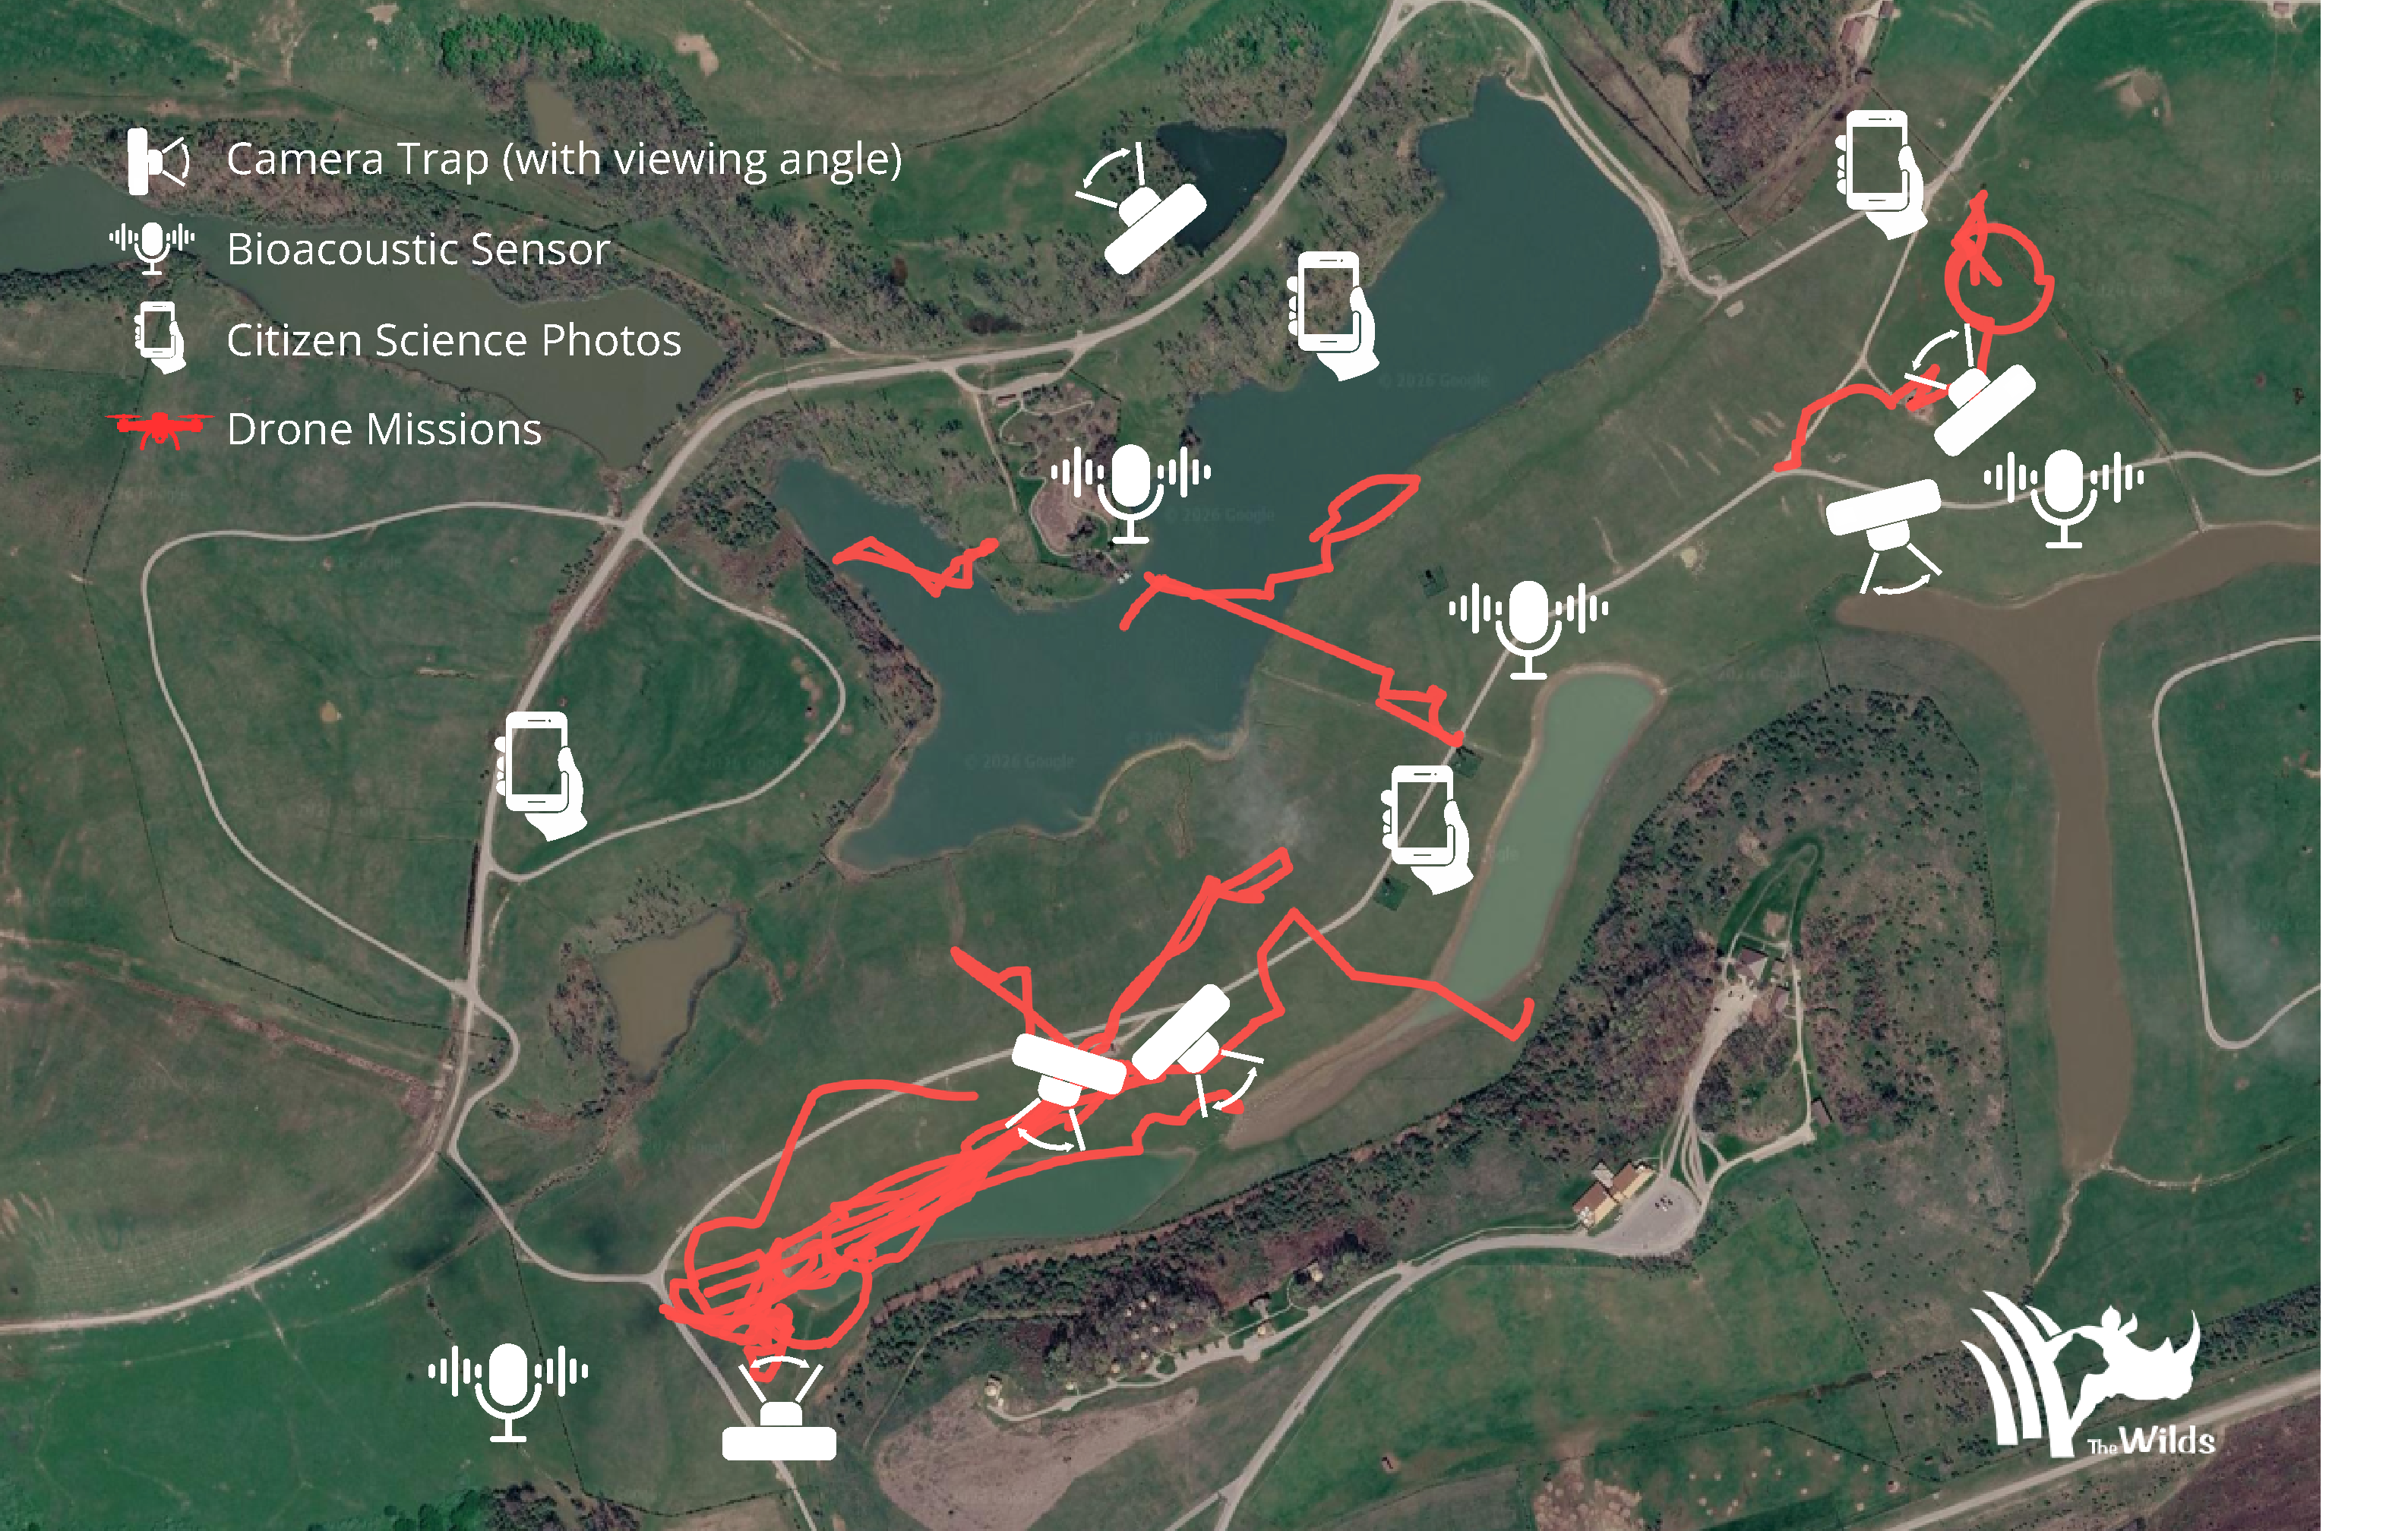
\includegraphics[width=0.84\textwidth]{figures/smartwildsmap.pdf}
    \caption{\smartwilds sensor deployment across the study area. Camera
    traps are shown with their viewing angles, Song Meter recorders at
    their fixed positions, drone flight tracks in red, and
    citizen-science records at locality level. The four modalities
    differ in spatial support as well as cadence: cameras and recorders
    sample fixed points, drone tracks sweep the pastures and lake
    margin, and citizen-science records resolve only to a locality.
    Satellite imagery \copyright\ Google.}
    \label{fig:map}
\end{figure*}

\subsection{Data Collection Campaign}

Data collection comprised three campaigns (Table~\ref{tab:campaigns}):
a four-day pilot (2025-06-30 to 07-03) that established site selection,
mounting, and configuration practice; the main deployment
(2025-08-04 to 08-28), a 24-day span over 25 calendar dates with all
four modalities, nine camera installations, six recorder deployments,
and drone flights on three dates; and a single-day drone revisit
(2025-09-08) with a different platform. All characterization in
\S\ref{sec:characterization} uses Campaign~2, the only window in which
all modalities were simultaneously active.

\begin{table}[t]
\caption{Campaign structure and raw data volume. Volumes are
on-disk sizes in the project archive.}
\label{tab:campaigns}
\small
\begin{tabular}{llrrr}
\toprule
& & \textbf{C1} & \textbf{C2} & \textbf{C3} \\
\midrule
\multicolumn{2}{l}{Start} & 2025-06-30 & 2025-08-04 & 2025-09-08 \\
\multicolumn{2}{l}{End} & 2025-07-03 & 2025-08-28 & 2025-09-08 \\
\multicolumn{2}{l}{Calendar dates} & 4 & 25 & 1 \\
\midrule
\multirow{2}{*}{Camera traps} & GB & 49 & 211 & --- \\
 & files & 20{,}027 & 220{,}898 & --- \\
\multirow{2}{*}{Bioacoustics} & GB & 6.0 & 196 & --- \\
 & files & 318 & 2{,}157 & --- \\
\multirow{2}{*}{Drones} & GB & 46 & 33 & 11 \\
 & files & 35 & 20 & 22 \\
\multirow{2}{*}{Citizen science} & GB & --- & 9.4 & --- \\
 & files & --- & 1{,}103 & --- \\
\midrule
\multicolumn{2}{l}{\textbf{Total (GB)}} & \textbf{101} & \textbf{449} & \textbf{11} \\
\bottomrule
\end{tabular}
\end{table}

\subsection{Sensing Modalities and Configurations}

We deployed deliberately \emph{heterogeneous} hardware. The resulting
configuration diversity is the largest single source of downstream
metadata work, and it is why the configuration tables are part of the
release.

\begin{figure*}[t]
    \centering
    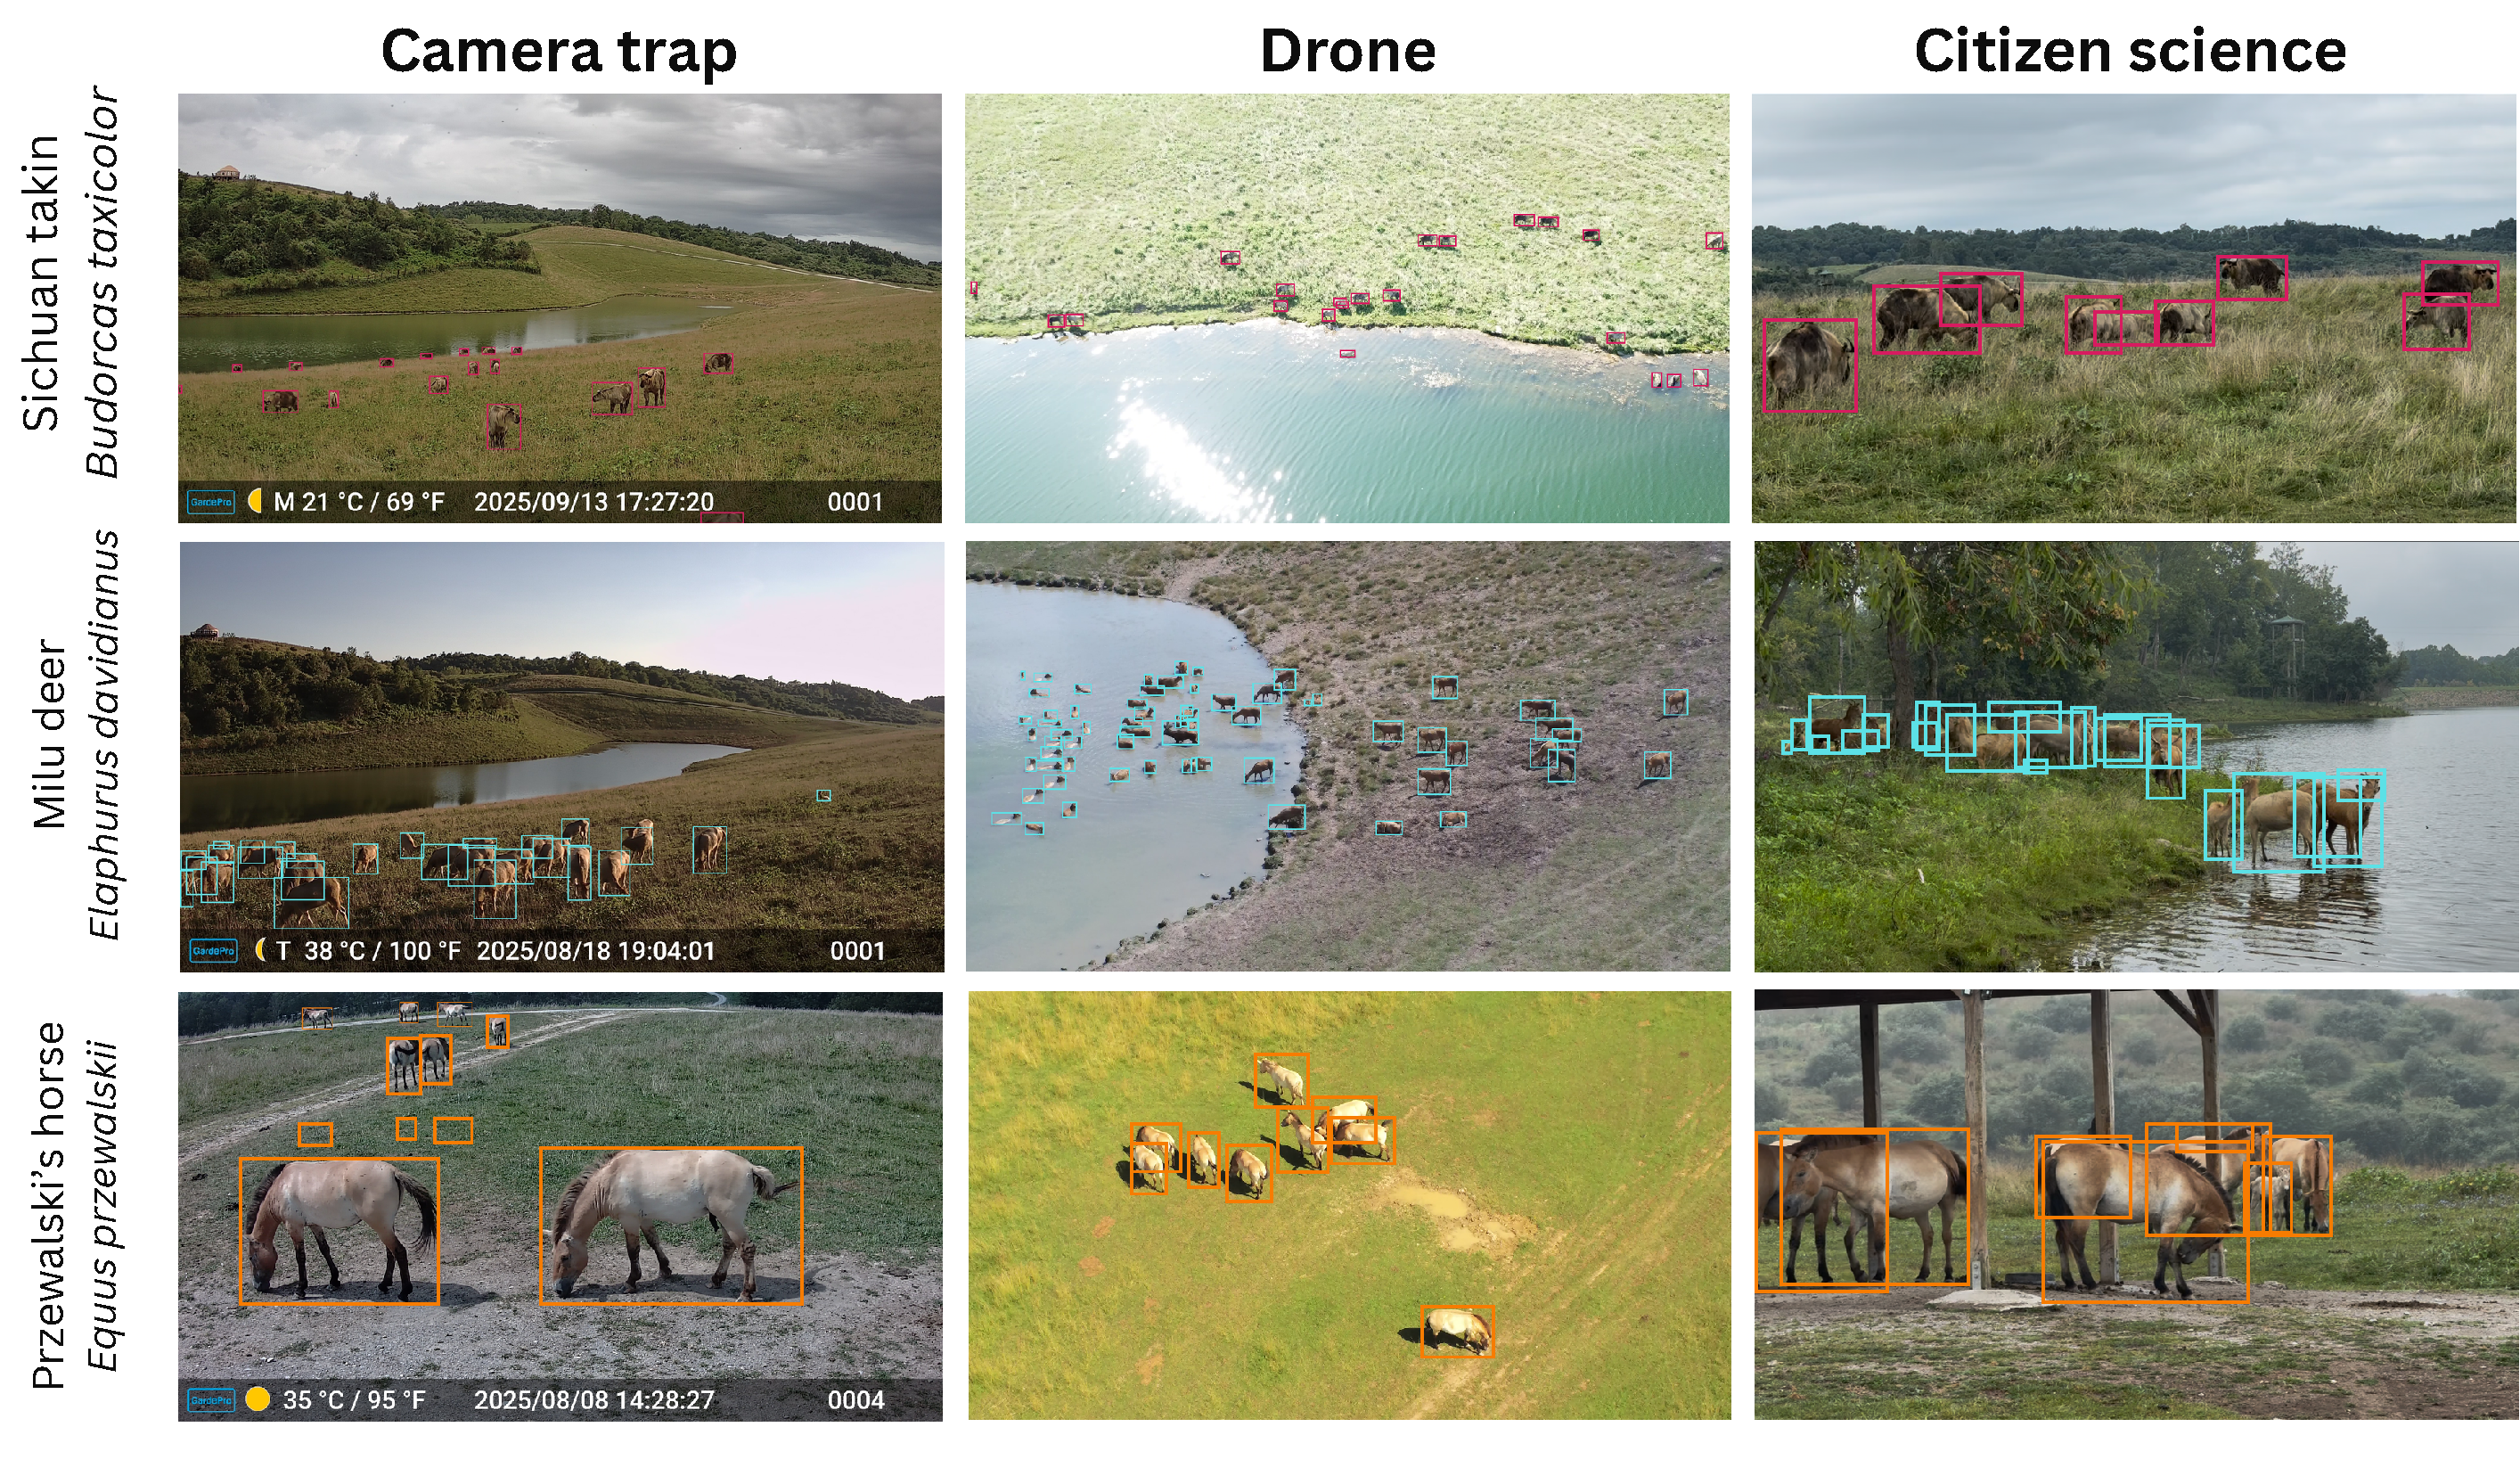
\includegraphics[width=0.88\textwidth]{figures/datapreview.pdf}
    \caption{The same three managed focal species --- Sichuan takin,
    Milu (P\`ere David's) deer, and Przewalski's horse --- as observed by
    camera trap, drone, and citizen-science photography, with SAM3
    detections. The modalities differ in viewpoint, scale, and
    resolution as much as in cadence. Camera-trap overlays show the
    device's raw clock, not the corrected timestamp: the takin frame's
    overlay reads 2025/09/13 for an image captured in August
    (\S\ref{sec:timestamps}).}
    \label{fig:preview}
\end{figure*}

\subsubsection{Camera traps}
Thirteen deployments used four camera models with horizontal fields of
view from 55$^\circ$ to 120$^\circ$, varying in capture mode (photo-only,
photo+video, hybrid with hourly timelapse), resolution (4\,MP, 8\,MP,
4K), burst length (3 or 5 frames per trigger), PIR sensitivity, and
inter-trigger delay (0--20\,s). One model is cellular-capable, making it
the only device here that could in principle participate in
near-real-time coordination.

Each parameter is a workload multiplier: a 5-frame burst produces five
times the raw images per ecological event as a single capture, a 20\,s
delay suppresses repeat triggers and lowers the effective arrival rate,
and video mode adds a 10--15\,s clip per trigger with disproportionate
storage and frame-extraction cost. The 13 deployments yielded
235{,}778 still images and 5{,}113 video clips, distributed extremely
unevenly: one dock-facing deployment produced 90{,}834 images, 38.5\% of
the total, while four produced fewer than 100 each. Per-deployment
models, configurations, and counts are in the supplement.



\subsubsection{Bioacoustics}
All acoustic recording used Wildlife Acoustics Song Meter Micro 2 units
at 48\,kHz. Ten deployments across six sites produced 2{,}453 WAV files.
Duty cycles differed deliberately: 5\,min/hour (8.3\%), 15\,min/hour
(25\%), continuous sunrise-to-sunset (roughly 50--60\% seasonally), and
continuous 24/7. One Campaign~1 unit was misconfigured --- intended to
record one hour at sunrise and sunset, it instead recorded 5-minute
clips hourly --- an error we discovered only from the resulting file
inventory.

Duty cycle dominates acoustic storage, since uncompressed 48\,kHz stereo
WAV runs roughly 33\,MB/minute. The two sunrise-to-sunset units each
produced over 56\,GB in 24 days, while the 5\,min/hour unit produced
26\,GB from more than twice as many files --- file count and byte volume
are independent axes. Per-deployment schedules, GPS positions, and
counts are in the supplement.



\subsubsection{Drones}
Drone survey used three platforms: a Parrot Anafi 4K (10 video-bearing
sessions across both campaigns; three additional Aug.~25 directories contained
metadata but no video; 4K MP4 video with Parrot JSON / GUTMA DX telemetry),
an unspecified DJI airframe (one Campaign~2 session,
1080p MOV with 10\,Hz CSV telemetry), and a DJI Air 2 (four Campaign~3
flights, 4K MP4 with Airdata CSV telemetry). The three platforms
produced three telemetry schemas with different field names, units
(feet vs.\ meters for altitude), and gimbal-angle conventions ---
a reconciliation cost documented in \S\ref{sec:scope}.

\subsubsection{Citizen science and text records}
Park visitors submitted photographs and observations through a
structured web form, yielding 1{,}103 raw-folder media files. Manual annotation
covered 791 photos and retained 564 wildlife photos, which yield 622 taxon
Occurrences; 50 curated September 8 photos are Google Photos album-export assets
outside the raw folder. Visitor submissions arrive only within operating hours,
producing the sharply truncated
diurnal profile in \S\ref{sec:characterization}. We additionally
curated a small set of text-derived records from field notes and
site-selection rationale, which we retain as a distinct modality
because they carry the human reasoning behind sensor placement.

\subsection{Field Protocol and Human Workflow}

Each cycle involved site selection, mounting and configuration,
periodic servicing, SD-card retrieval, transfer to institutional
storage, and logging. Two structured field logs, camera-trap and
bioacoustic, were captured through forms during Campaign~2; they are the
metadata most relied on in the release (\S\ref{sec:redundancy}). Human effort concentrated in two places we did
not anticipate: SD-card handling, where one camera's data arrived split
across several cards with inconsistent clock states, and the timestamp
reconstruction of \S\ref{sec:timestamps}.

\subsection{Ethics, Permissions, and Sensitive Records}

All work was conducted with the permission and participation of The
Wilds. Two categories of sensitive content required handling. Visitor
imagery: the TW07-CT05 deployment captured only people on tour buses and
no wildlife. Its deployment note states that the camera was monitored
through the mobile app and that the people-only photos were not uploaded;
the release contains no image, Event, or Occurrence from this deployment.
The retained archive contains metadata only, so we make no claim about
whether images remaining on the device were later deleted. And locality precision: citizen-science
coordinates are generalized and records for sensitive taxa are reduced
in precision via Darwin Core \texttt{informationWithheld} and
\texttt{dataGeneralizations}.

% ============================================================
\section{Cross-Modal Data Model}
\label{sec:model}

\subsection{Terminology}
\label{sec:glossary}

Ecology, computer vision, and sensing systems overload the same small
set of words, and in a cross-modal release that ambiguity is a direct
source of analysis error. Table~\ref{tab:glossary} fixes our vocabulary.
The entry that matters most is \emph{Event}: in Darwin Core a sampling
act with a location, date, and
protocol~\cite{wieczorek2012darwincore,tdwgDarwinCore}; in sensing
systems an arrival in a stream. They are not in correspondence --- one
Darwin Core Event, a 24-day camera deployment, contains tens of
thousands of image captures. We keep the Darwin Core meaning for the
record types we release and the FAIR\textsuperscript{2} Drones
conventions for effort and platform
metadata~\cite{pierrat2025proximal}, and say \emph{arrival} for the
systems sense.

\begin{table*}[t]
\caption{Terms this release overloads, with the sense used here. The
full glossary, including \texttt{eventType}, \texttt{basisOfRecord},
duty cycle, detection, identification, and coverage, is in the
supplement.}
\label{tab:glossary}
\footnotesize
\begin{tabular}{p{0.13\textwidth}p{0.07\textwidth}p{0.38\textwidth}p{0.34\textwidth}}
\toprule
\textbf{Term} & \textbf{Source} & \textbf{Definition} & \textbf{Note} \\
\midrule
\textbf{Event} & DwC & A sampling act: a camera deployment, one WAV recording, one flight session, one drone video, one observation session. Has a date, location, protocol, and \texttt{parentEventID}. & Not an arrival in a stream, and not a detection. One Event can contain $10^5$ arrivals. \\
\textbf{Occurrence} & DwC & One organism record at a place and time, linked to an Event by \texttt{eventID}. Usually one detection crop. & Not an individual animal: adjacent drone frames yield many Occurrences of the same animal. \\
\textbf{Arrival} & systems & One item entering a processing stream. Two layers measured: \emph{acquisition} (an image capture, a WAV file) and \emph{detection} (an Occurrence emitted by the detector). & Not a DwC Event. \\
\textbf{Sampling effort} & Humboldt & Acquisition actually expended: camera observation-days, recorder-hours, flight-minutes, visitor sessions. Reported per modality, never summed. & Not comparable across modalities, and not a detection count. \\
\textbf{\texttt{locationID}} & DwC & Stable identifier for a \emph{fixed} sensor position or a drone session origin; null for locality-only records. & Not a comparable spatial sampling unit across modalities (\S\ref{sec:identifiers}). \\
\textbf{Verification status} & DwC & Per-record: \texttt{unverified} (550{,}722), \texttt{validated} (1{,}590), \texttt{verified by expert} (652). & Not a confidence score; \texttt{validated} means a person reviewed it. \\
\bottomrule
\end{tabular}
\end{table*}

\subsection{Design Requirements}

The model serves two audiences: ecologists want Darwin Core records they
can push to GBIF, systems researchers want device schedules, trigger
semantics, and failure records. Rather than maintain two releases we use
Darwin Core as the interchange layer and extend it, keeping every
systems field in a named column rather than in prose. Four requirements
drove the design --- \emph{heterogeneity}, so fixed sensors and moving
platforms are first-class rather than special cases of each other;
\emph{traceability}, so every Occurrence resolves to a device, a time
reference, a spatial reference, and a transformation chain;
\emph{explicit uncertainty}, so estimated quantities are distinguishable
from observed ones per record rather than per dataset; and
\emph{extensibility}, so a fifth modality does not require re-keying the
first four.

\subsection{Four-Level Event Hierarchy}

Events form a four-level tree (Figure~\ref{fig:hierarchy}):

\begin{description}
\item[Study.] One root event, \texttt{TheWilds\_2025}, spanning the full
campaign extent (2025-06-30 to 2025-09-08) with a coarse study-area
coordinate and 5\,km uncertainty.
\item[Project.] One per modality (camera traps, bioacoustics, drones,
citizen science, text data), carrying the modality's sampling protocol
and aggregate sample size.
\item[Deployment / session.] One per physical installation or mission:
\texttt{SensorDeployment} for the 12 retained camera installations and
10 recorder deployments, and for the 15 video-bearing drone flight sessions. These
carry fixed coordinates (5\,m uncertainty) for stationary sensors,
device model and serial, schedule, and deploy/retrieve dates.
\item[Capture.] One per acquisition unit below the deployment:
2{,}371 \texttt{AudioRecording} events (one per processed WAV file,
with start time and duration, including 64 recordings on which BirdNET
emitted no detection), 39 \texttt{MediaEvent} events (one per raw drone
video, including one reviewed and excluded video with no Occurrences),
and 17 \texttt{ObservationSession} events for citizen-science and text
records.
\end{description}

The resulting table holds 2{,}470 Darwin Core Events
(Table~\ref{tab:schema}). Occurrences attach to the lowest available
level via \texttt{eventID}, so an acoustic detection resolves to a
specific WAV file while a camera-trap detection resolves to a deployment
interval. The asymmetry is deliberate: flattening it would fabricate
acquisition-boundary precision the cameras do not provide.

\begin{table}[t]
\caption{Darwin Core Event hierarchy and Occurrence counts in the
released snapshot (\texttt{darwin\_core\_\allowbreak latest\_\allowbreak 20261008}). Hourly bins count
distinct (date, hour) pairs containing at least one Occurrence, over
the full study extent (2025-06-30 to 2025-09-08). The 2025-08-11 drone
session carries a date but no time (\S\ref{sec:nulldefect}), so it
counts toward drone dates but not bins.
\TODO{Camera dates/bins (29 / 624) assume the 439 curated camera
Occurrences are re-timed from the corrected timestamp map; the current
snapshot gives 30 / 625.}}
\label{tab:schema}
\small
\begin{tabular}{lrrrr}
\toprule
\textbf{Modality} & \textbf{Events} & \textbf{Occ.} & \textbf{Dates} & \textbf{Bins} \\
\midrule
Study root & 1 & --- & & \\
Camera traps & 13 & 224{,}149 & 29 & 624 \\
Bioacoustics & 2{,}382 & 9{,}960 & 29 & 650 \\
Drones & 55 & 318{,}203 & 6 & 8 \\
Citizen science & 14 & 622 & 13 & 28 \\
Text data & 5 & 30 & 4 & 4 \\
\midrule
\textbf{Total} & \textbf{2{,}470} & \textbf{552{,}964} & & \\
\midrule
\multicolumn{5}{l}{\emph{By \texttt{eventType}}} \\
\texttt{Project} & 6 & & & \\
\texttt{SensorDeployment} & 37 & & & \\
\texttt{AudioRecording} & 2{,}371 & & & \\
\texttt{MediaEvent} & 39 & & & \\
\texttt{ObservationSession} & 17 & & & \\
\bottomrule
\end{tabular}
\end{table}

\begin{figure}[t]
    \centering
    \resizebox{\linewidth}{!}{% SmartWilds release schema (ER-style). Darwin Core core tables: dark headers.
% SmartWilds extension tables: light headers. Arrows point from FK to PK.
\begin{tikzpicture}[
  font=\scriptsize,
  tbl/.style={draw, rectangle split, rectangle split parts=2,
              rectangle split part fill={#1,white}, inner sep=2pt,
              align=left, rounded corners=1pt},
  core/.style={tbl=black!75, text width=3.75cm},
  ext/.style={tbl=black!15, text width=3.45cm},
  fk/.style={-{Latex[length=1.5mm]}, semithick},
  lbl/.style={font=\tiny\itshape, inner sep=0.8pt},
]
\newcommand{\pk}[1]{\underline{#1}}
% ---------------- Darwin Core core (left column) ----------------
\node[core] (ev) at (0,0) {\textcolor{white}{\textbf{Event}\hfill 2{,}470 rows}
  \nodepart{two}\raggedright
  \pk{eventID}\\
  parentEventID $\rightarrow$ Event\\
  eventType (4 levels)\\
  eventDate, eventTime\\
  lat, lon, uncertainty\\
  samplingProtocol, sampleSize\\
  fieldNotes (provenance)};
\node[core, below=4mm of ev] (oc) {\textcolor{white}{\textbf{Occurrence}\hfill 552{,}964 rows}
  \nodepart{two}\raggedright
  \pk{occurrenceID}\\
  eventID $\rightarrow$ Event\\
  taxon ranks, basisOfRecord\\
  identifiedBy (model, version)\\
  verificationStatus\\
  remarks: score, box, status\\
  coordinates + generalization\\
  associatedMedia $\rightarrow$ Media};
\node[ext, below=4mm of oc] (arr) {\textbf{Arrival traces}
  \nodepart{two}\raggedright
  sourceID $\rightarrow$ Occ. $|$ Event\\
  layer, timestamp, eligibility};
% ---------------- SmartWilds extensions (right column) ----------------
\node[ext, anchor=north west] (dep) at ([xshift=6mm]ev.north east) {\textbf{Deployment settings}
  \nodepart{two}\raggedright
  deploymentID $\rightarrow$ Event\\
  model, HFOV, bearing\\
  schedule, trigger, burst};
\node[ext, below=2.5mm of dep] (rec) {\textbf{WAV reconciliation}
  \nodepart{two}\raggedright
  eventID $\rightarrow$ Event\\
  path, status, disposition};
\node[ext, anchor=north west] (det) at ([xshift=6mm, yshift=-1mm]oc.north east) {\textbf{Drone detections}
  \nodepart{two}\raggedright
  occurrenceID $\rightarrow$ Occ.\\
  video, frame\_index, box};
\node[ext, below=2.5mm of det] (med) {\textbf{Media manifest}
  \nodepart{two}\raggedright
  \pk{release\_path}\\
  bytes, include flag\\
  exclusion reason\\
  has\_human\_detection};
\node[ext, below=2.5mm of med] (img) {\textbf{Image timestamps}
  \nodepart{two}\raggedright
  release\_path $\rightarrow$ Media\\
  raw ts + source\\
  corrected ts, method\\
  confidence};
% ---------------- relationships (FK -> PK) ----------------
\draw[fk] ([yshift=-1.5mm]ev.two west) -- ++(-3mm,0) |- node[lbl, left, pos=0.25] {self} ([yshift=1.5mm]ev.text west);
\draw[fk] (oc.north) -- (ev.south);
\draw[fk] (arr.north) -- (oc.south);
\draw[fk] (dep.west) -- (dep.west -| ev.east);
\draw[fk] (rec.west) -- (rec.west -| ev.east);
\draw[fk] (det.west) -- (det.west -| oc.east);
\draw[fk] (med.west -| oc.east) -- node[lbl, above] {media} (med.west);
\draw[fk] (img.north) -- (med.south);
\end{tikzpicture}
}
    \caption{Release schema. Darwin Core core tables (dark) and
    \smartwilds extension tables (light); arrows run from foreign key to
    primary key. The Event table is self-referencing and encodes the
    four-level hierarchy (study $\supset$ modality project $\supset$
    deployment or session $\supset$ capture), so fixed sensors and moving
    platforms both sit at the deployment level and a cross-modal query
    over a time window returns both without special-casing. Extension
    tables carry what Darwin Core cannot: sensor settings, timestamp
    provenance, media inclusion and privacy status, frame-level drone
    detections, per-file acoustic disposition, and versioned arrivals.}
    \label{fig:hierarchy}
\end{figure}

\subsection{Identifiers and Spatial Semantics}
\label{sec:identifiers}

Identifiers encode what kind of thing they name: fixed sensor
deployments use \texttt{TW\{site\}-\{device\}\_\{start\}\_\{end\}},
drone sessions \texttt{\{date\}\_\{platform\}\_\{seq\}}, and capture
Events append the acquisition identifier --- a convention that later
turned out to be error-correcting (\S\ref{sec:nulldefect}).
\texttt{locationID} is populated \emph{only} for fixed sensor sites
(7 camera, 6 recorder) and drone session origins (15); citizen-science
records carry a locality name and a null \texttt{locationID}. This is the most consequential typing decision in
the schema: a \texttt{GROUP BY locationID} cannot present 15 drone
session origins and 7 fixed camera positions as comparable sampling
units, because the semantics are documented per modality and the
locality-only rows are null rather than coerced.

Spatial support differs by modality and is recorded as such.
Deployment-level coordinates are sensor positions with 5\,m uncertainty.
Occurrence-level coordinates are estimated positions for camera traps
and drones, recorder positions for acoustics, and generalized localities
for citizen science; every Occurrence carries
\texttt{coordinateUncertaintyInMeters} and a
\texttt{dataGeneralizations} string saying which it is.

\subsection{Semi-Automated Analysis}
\label{sec:provenance}

A sensor network of this size forecloses manual annotation. The release
holds 235{,}778 images, 5{,}113 video clips, 2{,}453 acoustic
recordings, and 39 drone videos; our human-reviewed subsets are 0.4\% of
it and consumed the review capacity we had. Scaling that to the full
release is a structural limit rather than a funding one, and it tightens
with every deployment: data volume grows with devices and duty cycle
while expert review capacity does not.

We therefore treat semi-automated analysis as the operating condition
for sensor-network data rather than as a compromise, and instrument it
accordingly, using current state-of-the-art models ---
SAM3~\cite{carion2026sam}, BioCLIP
Tree-of-Life~\cite{stevens2024bioclip,gu2025bioclip,treeoflife_200m},
and BirdNET~\cite{kahl2021birdnet} --- so that reported quality reflects
what a practitioner adopting today's best tooling would obtain. A weaker
detector would understate what is achievable; hand-curated labels would
overstate it, and would describe a workflow that does not scale.

Every visual Occurrence is accordingly a three-stage output: SAM3
produces a box, BioCLIP Tree-of-Life a top-1 taxon with full rank
hierarchy, and a projection script an estimated coordinate
(\S\ref{sec:scope}). Acoustic Occurrences come from BirdNET detections
with frequency bounds and an offset into the source WAV. Following
scientific-workflow provenance practice~\cite{simmhan2005provenance}, the chain is
recorded per record in \texttt{identificationRemarks} and
\texttt{occurrenceRemarks}, with scripts and configurations copied into
the release beside the data.

\subsection{Model Identity, Uncertainty, and Reproducibility}
\label{sec:modelprov}

If a dataset's labels are model outputs then the model is part of the
data, and omitting it is comparable to omitting the sensor
specification. Current practice in both ecological and computer-vision
releases often publishes none of it. Four reasons to do so follow.

\emph{A taxon label is not reproducible without its model.} Two versions
of the same classifier yield different taxa from the same image, so a
release stating ``\emph{Elaphurus davidianus}'' without stating what
produced the string gives a reader no experiment that should recover the
table. Model identity, version, weights provenance, and inference
parameters are the minimum for reproducing or auditing the labels.

\emph{Published uncertainty is what makes labels re-derivable.} Machine
labels are a snapshot of a model, not ground truth, and will be
superseded. A release keeping source media, detection geometry, model
identity, and per-rank accuracy can be \emph{re-labeled} when better
models arrive, with old and new sets compared meaningfully; one shipping
only final taxon strings cannot. This is the main practical reason to
publish the chain.

\emph{Aggregate accuracy obscures the rank-dependent failure mode.}
Accuracy does not degrade uniformly with rank. On our human-annotated
camera-trap subsets, localization is strong (precision 0.866, recall
0.845, F1 0.856 at IoU $\geq 0.50$, $n{=}1{,}125$) while taxonomic
assignment collapses ($n{=}951$): 0.845 at class, 0.660 at order,
0.463 at family, 0.322 at genus, 0.271 at species. A single headline number in that range would
not be informative. The usable statement is structural ---
class-rank labels support screening, species-rank labels require
curation, and aggregating across ranks is uninterpretable. The taxonomy
crosswalk agrees from the other direction: of 12{,}577 label keys only 4
consist entirely of expert-verified records.

\emph{Verification status must be per record.} A README caveat cannot be
filtered on, so \texttt{identification\allowbreak Verification\allowbreak Status} is carried on
every row: 550{,}722 (99.6\%) \texttt{unverified} machine predictions,
1{,}590 \texttt{validated} by human review (946 camera-trap and 644
drone bird records from a targeted review set), and 652
\texttt{verified by expert} (all citizen-science and text records).
\texttt{basisOfRecord} separates 552{,}312 \texttt{MachineObservation}
rows from 652 \texttt{HumanObservation} rows. A user wanting only
human-verified data gets it with one predicate; a user training on
machine labels and evaluating on verified ones can build that split
correctly instead of accidentally mixing them. In our own use, disagreements about
results most often traced back to two people assuming different
verification floors.

\subsection{Missingness as Data}

The schema distinguishes six states that would otherwise collapse into a
single absence:

\emph{(1) Sensor active, nothing observed}, recoverable from the
deployment interval and schedule: an hourly bin inside a deployment
window with no Occurrence means the sensor was on and did not detect.
\emph{(2) Sensor inactive by schedule} --- the 5\,min/hour recorders are
off 91.7\% of the time by design, which the deployment-level schedule
field makes computable, as acquisitional sensor
databases require~\cite{madden2005tinydb}. \emph{(3) Sensor inactive by failure}, such as
battery exhaustion at TW02-CT01 (Aug 18--25), recorded as a gap with a
cause. \emph{(4) Captured but not represented}: of 2{,}453 WAV paths on
disk, 2{,}371 are \texttt{AudioRecording} Events; 78 are Campaign-1
files copied into a Campaign-2 directory during transfer and are
duplicates rather than recordings, and 4 produced no BirdNET result
(three 3.9--22.0\,s fragments and one unreadable file). A one-row-per-path
reconciliation table records the class of every file, and 64 processed
recordings with zero detections are retained as Events with no
Occurrences, so ``processed, nothing heard'' is distinguishable from
``not processed''.
\emph{(5) Metadata unusable for a purpose}: 41{,}524 drone Occurrences
(13.1\%) carry a date recovered from their identifier but no time of
day (\S\ref{sec:nulldefect}), and separately
70{,}219 detections cannot support per-animal ground projection and
retain platform coordinates with a status code (\S\ref{sec:scope}) ---
adequate for the campaign's purpose, unusable for one it was not
collected for. \emph{(6) Excluded in QC}: the people-only TW07-CT05
deployment is excluded and documented as such, so its absence does not
read as a site with no wildlife; one drone video, reviewed and found to
contain no usable content, is retained as a \texttt{MediaEvent} with no
Occurrences for the same reason.

States (1) and (2) have opposite implications for a coordination policy,
which is why the schedule field is required rather than descriptive.

\subsection{Standards Alignment}
\label{sec:crosswalk}

Darwin Core and its Humboldt extension~\cite{tdwgHumboldt} cover
taxonomic and Event structure well, and we reuse them directly for
taxon, date, coordinate, uncertainty, verification status, and effort
terms. We adopt the FAIR\textsuperscript{2} Drones card as the
documentation template~\cite{pierrat2025proximal}, express device
specifications in the spirit of SensorML~\cite{ogcSensorML} and
derivation in the spirit of PROV-DM~\cite{w3cProvDM} without encoding
either, and follow FAIR, CARE, and TRUST for
release~\cite{wilkinson2016fair,carroll2020care,lin2020trust}.

Six classes of information required for cross-modal reuse are
expressed by no standard we found in a machine-readable way: per-device
duty cycle and acquisition schedule; trigger semantics such as PIR
sensitivity, burst length, and inter-trigger delay; timestamp confidence
and repair method; per-detection coordinate provenance status; typed
missingness; and model identity with per-rank accuracy. We have named
these, used them consistently, and documented them, and we offer them as
a starting point for community work rather than a finished
specification. The full crosswalk is in the supplement.

% ============================================================
\section{Quality Control}
\label{sec:qc}

We encountered 20 defect classes. Table~\ref{tab:defects} groups them
by what each was \textbf{detected by}, because that is what determined
whether we could repair it; the full per-class inventory, with scope,
repair, and residual risk, ships with the release.

None of these classes is novel. Clock error, battery failure,
misconfiguration, and media fragmentation are documented hazards of
camera-trap and recorder
deployment~\cite{lahozmonfort2021monitoring,ahumada2020wildlifeinsights,Pestell2025SmartCamera},
and we encountered most of them. We organize the inventory by detection
source because detectability, rather than device reliability, is what
separated the repairable defects from the permanent ones; the release
inventory quantifies both the repairs and the residual uncertainty.

\begin{table}[t]
\caption{Defect classes by what made them detectable. All 20 classes,
with scope, repair, and residual risk, are inventoried in the release
(\texttt{metadata/DEFECT\_INVENTORY.md}) and supplement~S16.}
\label{tab:defects}
\small
\begin{tabular}{p{0.38\linewidth}rp{0.40\linewidth}}
\toprule
\textbf{Detected by} & \textbf{Classes} & \textbf{Example} \\
\midrule
External record (service log, field note, platform docs) & 5 & Wrong or unset camera clocks (93.9\% of images) \\
Redundant encoding in the data & 2 & \texttt{nan} date recovered from the \texttt{eventID} \\
Cross-check between artifacts & 8 & 146 WAV files with no \texttt{AudioRecording} Event \\
Human inspection & 3 & Visitor-only camera deployment \\
\midrule
None (fact recorded once) & 2 & Within-card clock drift \\
\bottomrule
\end{tabular}
\end{table}

\subsection{Detectability and Redundancy}
\label{sec:redundancy}

Eighteen of the twenty defect classes (Table~\ref{tab:defects}) were
repairable, and in every case the repair was possible because the fact
the device got wrong had been recorded somewhere a second time. The
general property is \emph{redundancy} rather than independence: two of
the six sources below sit inside the data the pipeline itself produced,
and they worked as well as the external ones. The six fall into four
families --- records external to the device, redundant encodings within
the data, cross-checks between two artifacts, and human inspection ---
and all six are cheap to produce at deployment time:

\begin{description}
\item[Service and deployment logs.] Two structured field logs from
Campaign~2 record when each device was deployed, serviced, and
retrieved --- the sole reason the clock defects were repairable, since a
camera asserting 2023 is correctable only against an external claim
about when it was in the field. Cost: minutes per visit.

\item[Field notes on deployment changes.] A free-text note that
TW09-CT02 moved from the dock to Nomad Ridge W on Aug 18 turned
90{,}834 images from one mislocated block into two correctly located
intervals; nothing in the device's output indicated the move. Cost: one
sentence.

\item[Cross-checks.] Comparing disk against pipeline output caught the
misconfigured recorder schedule, 146 unrepresented WAV files, and an
unprocessed drone video --- free, but only if raw media are retained
beside derived products.

\item[Redundancy in device output.] Three camera models burn the
timestamp into the image. For 182 images with no surviving filename or
EXIF timestamp, that pixel-level duplicate was the only record,
recoverable by OCR. This is the lowest-cost redundancy in the
deployment, and the vendor rather than the field team supplied it.

\item[Redundancy in identifiers.] Our \texttt{eventID}
convention embeds the acquisition date. When an entire drone session's
\texttt{eventDate} was written as the string \texttt{nan}, the
identifier was the only surviving record of when the flight happened
(\S\ref{sec:nulldefect}). We adopted the convention for readability and
got error correction free.

\item[Human review.] The inverted mount and the visitor-only deployment
were caught by a person looking at images. Automated checks catch
referential and format defects; semantic defects need eyes.
\end{description}

The two unrepaired rows define the boundary, and in both the relevant
fact was recorded exactly once. Within-card clock drift is unmeasurable because
we have exactly one external time anchor per card; a second anchor at
retrieval would have bounded it. True camera-days are unreportable
because the deployment metadata are themselves the only record of
deployment timing and contain known errors with nothing to check them
against. What is absent in both is a \emph{second} record of the same
fact, in any form.

We therefore state the requirement as redundancy rather than
reliability. Trail-camera clocks cannot be made trustworthy, but their
untrustworthiness can be made detectable and correctable by recording
the same fact twice from two sources. Where a second record existed we
recovered the value; where it did not, the uncertainty is permanent and
propagates into every trace derived from the baseline, so we record it
per record rather than in a release note.

\subsection{Timestamp Reconstruction}
\label{sec:timestamps}

Camera-trap time is the defect class we can quantify most completely.
The phenomenon itself is well
documented~\cite{lahozmonfort2021monitoring}; we report its cost in this
deployment. In temporal-database terms, the device asserts a valid time
we cannot trust~\cite{jensen1999temporal}, so we keep the raw value and
the reconstructed one side by side, each with its source and
confidence.

Of 235{,}778 images, only 14{,}472 (6.1\%, two Campaign~1 deployments)
had timestamps we could accept as recorded; the remaining
221{,}306 required reconstruction through 18 deployment- and
card-specific methods. The raw source varied too: 193{,}096 images
carried a parseable timestamp in the filename, 42{,}500 in EXIF, and
182 only as pixels burned into the frame, recovered by OCR (179) or by
hand (3). Repair followed three patterns --- raw timestamps accepted
where the clock agreed with service-log deploy times; a constant offset,
in the worst case of two years, anchored to a logged deploy time; and
per-card anchors where a deployment's images arrived on several SD cards
with independent clock states, four of them for TW02-CT01's
61{,}217 images. The supplement lists all 18 methods with counts.

The procedure converged --- all 235{,}778 images mapped, none unmapped,
none flagged for review --- but it converged to \emph{documented
confidence rather than correctness}. Only 105{,}488 timestamps (44.7\%)
are high confidence, meaning verified correct or anchored to a logged
service event. The remaining 130{,}290 (55.3\%) are anchored
interpolations assuming a constant clock rate, which we cannot test
without an external reference. Every temporal analysis in
\S\ref{sec:characterization} and every trace derived from this baseline
inherits that assumption, so we record it per image rather than once in
a README, and a user can filter on it.

In total, 18 repair methods produced full coverage in which 55.3\% of
timestamps rest on an assumption no second anchor can test
(\S\ref{sec:effort}). Two external time anchors per storage medium --- at
insertion and at retrieval, a few bytes each --- would have reduced the
procedure to one offset-and-rate computation per card and bounded the
drift we cannot currently measure. That is requirement R2 in
\S\ref{sec:lessons}, an instance of R1.

\subsection{Spatial Resolution}
\label{sec:scope}

The drone campaigns were flown to estimate populations of the managed
focal species and to observe behavior in aerial video. That purpose
sets the spatial resolution the release offers, and because every drone
Occurrence carries a \texttt{decimalLatitude}, this section states what
that coordinate means.

\emph{Platform position is the operative spatial reference.} The Wilds is organized into large managed pastures with known
boundaries, so a detection tagged with the aircraft's position places
the animal in a specific pasture. For population estimation and most
biodiversity summaries that is the resolution the question requires:
counting a herd, or recording that it was in the lake pasture, does not
need a deer's coordinate to three metres. The release treats platform
position as a first-class, adequate reference rather than a degraded
fallback. Camera-trap coordinates work the same way, with the fixed
sensor position accurate to 5\,m; their Occurrence-level coordinates are
pinhole projections assuming flat ground and a uniform 0.9\,m target
height, which at a site holding geese through Père David's deer is the
dominant error term.

\emph{Per-animal ground projection is an optional refinement.} We
additionally compute a first-pass ground position by intersecting a
bounding-box ray with a flat ground plane from per-frame telemetry.
Telemetry supports it for 247{,}340 of 317{,}559 detections (77.9\%);
for the rest, altitude source, platform GPS, or near-level camera
geometry put the intersection out of range, and the record keeps
platform coordinates with a status code. Monocular distance estimation
from a moving camera to moving subjects is not established practice in
aerial wildlife survey, and the error budget here is dominated by
terrain relief, gimbal-pitch convention, altitude source, and
stabilization offset. We release the coordinates, the per-detection
status, and the scripts as a starting point for work that wants to
improve on them; results in this paper and its companions rest on
platform position.

\emph{The relevant failure} is not imprecision, which is documented and
appropriate to the task, but \emph{mixing two spatial semantics in one
analysis}. An internal audit found a spatial figure plotting projected
animal positions and platform positions together without distinguishing
them; 15.66\% of the plotted drone points were platform coordinates.
Both coordinate kinds are legitimate and answer different questions at
different resolutions, so combining them silently yields a figure
meaning nothing in particular. The status field existed and was correct;
the script did not read it. Carrying a provenance field is necessary but
not sufficient; it must also be difficult to bypass, so the release
ships a validator that fails when an analysis consumes drone coordinates
without constraining the status column.

\subsection{Sentinel Values and Validator Coverage}
\label{sec:nulldefect}

One defect passed our own quality control and reached a released
snapshot. The QC summary for \texttt{darwin\_core\_\allowbreak latest\_\allowbreak 20260724}
reported \texttt{missing\_\allowbreak eventDate=0} for every modality
table. It was wrong for drones: 41{,}524 Occurrences (13.1\% of drone
Occurrences), spanning five drone video Events and their two parent
deployment Events, carried an \texttt{eventDate} of \texttt{nan} --- the
literal string a dataframe export writes for a missing value. The check
tested for null and empty, and \texttt{nan} is neither; the same rows
have an empty \texttt{eventTime}. The same audit then found impossible
coordinates (\texttt{nan}, and longitudes near 500) on seven drone
Events, passed by the same presence-only checks.

The affected records are the entire 2025-08-11 session, across both the
DJI and Parrot airframes, and the defect propagated through every
temporal summary: \texttt{nan} was counted as a seventh drone ``date'',
and Campaign~2 drone arrivals could cover only two of the three flight
dates. We found it only because an arrival analysis failed to parse the
column.

The date was recoverable because our \texttt{eventID} convention encodes
it (\texttt{TheWilds\_2025\_drone\_20250811\_DJI\_01}). The current
snapshot restores \texttt{eventDate=2025-08-11} from the identifier,
records in the remarks that the date is identifier-derived, and leaves
\texttt{eventTime} blank: neither the DJI telemetry nor the video
containers retain a trustworthy capture time, and we do not synthesize
one from file modification times. These records can be placed on a day
but not within it, and they are excluded from inter-arrival
statistics. A naming convention adopted for readability reduced a total
loss to a partial one, and the field that was not redundantly encoded is
unrecoverable.

Two generalizable points follow, both consistent with the
error-detection literature~\cite{abedjan2016detecting,schelter2018deequ}.
\emph{Validate types and domains, not just presence}: parse date columns rather than testing them for
emptiness, and fail the build on any string that will not parse.
Sentinels --- \texttt{nan}, \texttt{None}, \texttt{NULL}, \texttt{-1},
\texttt{1970-01-01} --- are normal dataframe output and will reach a
release unless something rejects them. And a passing validator bounds
what was checked, not what is correct: ours passed four structural checks
on 552{,}964 records while 13.1\% of one modality had no usable
timestamp. We therefore report validator coverage alongside validator
results.

\subsection{Validation and Snapshots}

The original four structural checks --- no missing event links, no
missing taxon, no missing event date, no duplicate Occurrence
identifiers --- were necessary but weak: they caught referential
breakage during development and missed the \texttt{nan} dates above.
The generator now parses every date, time, and coordinate pair and
rejects sentinel values before export, and the release audit checks,
over every modality and merged table: source-to-merged parity for Events
and Occurrences; a single-rooted Event hierarchy with no dangling
parents; Occurrence-to-Event links and ancestry; parsed dates, times,
and WGS84-bounded coordinates; resolvable media references; and
agreement between the generator and the released tables. The current
snapshot passes with zero errors and zero warnings.
\TODO{The audit does not yet check that an Occurrence date lies inside
its parent deployment interval; that check finds 439 curated camera
Occurrences (124 dated 2025-09-14, 315 with only the deployment
interval). Add the check, re-time them from the corrected map, and
re-run. Also re-verify media references: 10{,}943 drone Occurrences
still point at 479 scratch frames that have since been purged.}

We also adopted dated, immutable snapshots after an early mistake.
Analyses produced against one snapshot were compared against numbers
from another, and because the differences were \emph{semantic} rather
than additive --- different visual-label semantics, corrected timestamps
--- the comparison was invalid in a way invisible in the numbers. The
release now uses dated snapshot directories, retains before/after copies
of every mutation, and emits a JSON audit record per update; the
curated-bird update of 2026-09-20, which appended 946 validated
camera-trap and 644 validated drone records, is reconstructible from
three such files. Any figure must name the snapshot it came from.

% ============================================================
\section{Workload Characterization}
\label{sec:characterization}

This section establishes that \smartwilds supports workload
characterization, and reports the properties a practitioner needs in
order to judge whether the dataset fits their question. The full
treatment --- service demand, scheduling implications, trace generation
and replay --- is the subject of the companion workload
paper~\cite{smartwilds_workload}, and we do not duplicate it here.

Throughout, \emph{arrival} has its systems sense: one item entering a
processing stream (Table~\ref{tab:glossary}). All figures use Campaign~2
(2025-08-04 to 2025-08-28, 600 hours), the only window in which all four
modalities were simultaneously active, on the
\texttt{darwin\_core\_\allowbreak latest\_\allowbreak 20261008} snapshot. Every stream is released as a
versioned trace with a source-record identifier per arrival, the
inclusion rule, and input checksums; earlier unversioned arrival
summaries are deprecated.

\subsection{Acquisition and Detection Layers}

The property that most determines the dataset's usefulness is that it
supports workload reconstruction at \emph{two} layers rather than one.
\textbf{Acquisition arrivals} are what a storage or transfer subsystem
sees: one image capture, one WAV recording. We reconstruct them from the
corrected camera timestamp map and the \texttt{AudioRecording} Event
times. \textbf{Detection arrivals} are what a consumer of inference
output sees: one Darwin Core Occurrence. We reconstruct them from the
Occurrence table. Most released sensing datasets support neither; those
that do support one.

Table~\ref{tab:arrivals} reports both, using the burstiness coefficient
$B = (\sigma-\mu)/(\sigma+\mu) = (\mathrm{CV}-1)/(\mathrm{CV}+1)$ over
inter-arrival times, which is $-1$ for perfectly periodic arrivals, $0$
for Poisson, and approaches $1$ for maximally bursty arrivals.

\begin{table}[t]
\caption{Campaign-2 arrival characterization at two layers
(\texttt{darwin\_core\_\allowbreak latest\_\allowbreak 20261008}, 600-hour window).
Rates are time-eligible arrivals over the fixed window; CV is over
sorted inter-arrival times. Detection streams count machine-derived
Occurrences only (curated review records excluded); acoustic
recordings include zero-detection WAVs. Drone detections cover
two flight dates; the 2025-08-11 session (41{,}524 Occurrences) has a
date but no time and is excluded (\S\ref{sec:nulldefect}).
Acquisition arrivals are not reconstructible for drones (frame times are
not retained) or citizen science (one submission per session). See
\cite{smartwilds_workload} for the full analysis.}
\label{tab:arrivals}
\small
\begin{tabular}{lrrrr}
\toprule
\textbf{Stream} & \textbf{Arrivals} & \textbf{Rate/hr} & \textbf{CV} & \textbf{$B$} \\
\midrule
\multicolumn{5}{l}{\emph{Acquisition layer}} \\
Camera captures & 220{,}697 & 367.83 & 2.06 & $+0.347$ \\
Acoustic recordings & 2{,}060 & 3.43 & 1.23 & $+0.103$ \\
\midrule
\multicolumn{5}{l}{\emph{Detection layer}} \\
Camera traps & 208{,}054 & 346.76 & 7.26 & $+0.758$ \\
Bioacoustics & 8{,}865 & 14.78 & 3.21 & $+0.525$ \\
Drones & 53{,}238 & 88.73 & 229.61 & $+0.991$ \\
Citizen science & 242 & 0.40 & 5.30 & $+0.682$ \\
\bottomrule
\end{tabular}
\end{table}

Three properties of the release follow.

\emph{Inference amplifies burstiness.} Wherever both layers are
measurable the detection stream is markedly burstier than the
acquisition stream feeding it --- camera traps $+0.347\!\to\!+0.758$,
acoustics $+0.103\!\to\!+0.525$ --- because most captures contain no
subject and the ones that do contain several. Any dataset used to
evaluate edge inference placement needs both layers; this one has them.

\emph{Sensing policy, not the subject, sets the acquisition regime.}
Acoustic acquisition is the deployment's most regular stream
($B{=}+0.103$, essentially Poisson) because the duty cycle dominates it
completely, while detections from the same files concentrate in the dawn
chorus ($B{=}+0.525$). Regularity from policy is \emph{controllable},
the lever an adaptive system pulls, and the release carries the
per-device schedules needed to model the counterfactual.

\emph{Volume and burstiness are decoupled.} Drone detections
($B{=}+0.991$) fall entirely within single flight hours at over
2{,}100 arrivals/hour against a 600-hour mean of 88.73, while camera
traps generate the most arrivals and are not the burstiest --- so a
scheduler optimizing throughput and one optimizing tail latency would
prioritize different modalities.

\subsection{Diurnal Structure}

Figure~\ref{fig:diurnal} shows hourly profiles at both layers, and the
layer distinction reappears. Camera \emph{captures} swing only
2.1$\times$ across the day (286 arrivals/hour at 23:00 to 612 at 13:00)
because the sensors stay on; camera \emph{detections} swing
12.5$\times$ (54 to 674). Acoustic acquisition is nearly flat at
4.3 recordings/hour, while acoustic detections peak at 41.6/hour at
06:00 against a 3.0 nocturnal floor, with a secondary dusk rise to 36.2
at 19:00. Citizen science is concentrated in 09:00--12:00; drone
detections are zero for 23 hours.

The profiles show the coordination opportunity directly: the modalities
with persistent coverage are active when those with high information
density per unit time are not, so a trigger from a
persistent sensor to a scarce one has more than 20 hours a day in which
it could do useful work.

\begin{figure}[t]
    \centering
    % \includegraphics[width=\linewidth]{figures/diurnal-profiles.pdf}
    \caption{Campaign-2 diurnal arrival profiles (log scale),
    acquisition layer dashed and detection layer solid. Detection
    profiles are sharper than the acquisition profiles that feed them in
    every modality where both are measurable.}
    \label{fig:diurnal}
\end{figure}

\subsection{Coverage}

Temporal and spatial coverage diverge sharply (Table~\ref{tab:schema}).
Over the full study extent, camera traps contribute Occurrences in
624 distinct hourly bins and acoustics in 650, against 8 for drones and
28 for citizen science --- roughly an 80$\times$ difference in temporal reach.
Spatially the ordering inverts: drones cover the pastures across
15 session origins, while camera traps observe from 7 fixed positions
through 55--120$^\circ$ apertures and recorders from 6. Persistent
modalities are active precisely when episodic, information-dense ones
are not, which is the structural basis for trigger-style coordination.

We deliberately do not reduce these to a single coverage number. Camera
observation-days, recorder-hours, flight-minutes, and visitor sessions
are different acquisition processes, and the denominators that would
make them comparable were never captured. A practitioner should treat
per-modality effort as the unit and normalize explicitly if they must
--- see requirement R6 in \S\ref{sec:lessons}.

\subsection{Storage and Data Movement}

Volume matters for reuse planning, so we state it here; the companion
workload paper treats the resulting service demand in
detail~\cite{smartwilds_workload}. Raw volume is dominated by two
modalities for different reasons (Table~\ref{tab:campaigns}). Camera
traps produce 260\,GB from 240{,}925 small files, so their cost is in
file count and per-file inference as much as in bytes, and they would
benefit from on-device filtering. Acoustics produce 202\,GB from
2{,}453 large files driven purely by duty cycle, making the duty cycle
the primary control knob. Drones produce 90\,GB from 39 videos, the
highest bytes-per-file by three orders of magnitude, arriving as a burst
with no chance of incremental processing unless the processing moves onto
the aircraft. All three were moved by physically carrying SD cards,
which is the deployment's dominant data-movement mechanism and its
dominant latency: days, not seconds.

\subsection{Human Effort}
\label{sec:effort}

Human effort is part of the baseline: a practitioner planning a
comparable deployment needs to budget for it, and no sensor
specification predicts it.

Field servicing is measured, because the Campaign-2 logs timestamp every
visit. Across three logged service trips (Aug 4, 7, and 11) the team
recorded 23 sensor servicing actions --- 11 deployments, 6 retrievals,
5 status checks, and 1 combined visit, split 12 acoustic and 11 camera
--- in 245 minutes of elapsed field time, or 4.1 hours. Per-trip elapsed
time was 103, 66, and 76 minutes, and the median interval between
consecutive sensor actions was 16 minutes on the first trip and
3 minutes on the later two. The logs also carry a 1--3 access-difficulty
rating, recorded for 15 of the 23 actions, plus battery and SD-card
status at each check. Servicing a mesoscale deployment of this size is
therefore a few hours of field time per trip, which is the figure to use
when sizing a comparable campaign. These logs cover the three
mid-campaign trips only: Campaign-1 field notes are narrative and carry
no clock times, and the Aug 28 retrieval visits are absent from the
exported forms.

Post-deployment effort is recorded only descriptively, and it
concentrated in three places a hardware budget would not anticipate:
timestamp reconstruction, which required developing 18
deployment-specific repair methods including manual reads of burned-in
overlays; telemetry reconciliation across three platform schemas; and
taxonomic review, which produced a 12{,}577-key crosswalk of which only
4 keys consist entirely of expert-verified records, with a 500-record
priority review queue still outstanding. Field visits were logged with
timestamps; processing stages were not, so this side is reported as
activities rather than hours. No retrospective analyst-hour estimate is
reported. Requirement R7 in \S\ref{sec:lessons} is to log both the same way.

% ============================================================
% ============================================================
\section{Instrumentation Requirements for Future Deployments}
\label{sec:lessons}

Each requirement below is written so a future deployment can verify it
has done it, and each comes from a specific defect in
Table~\ref{tab:defects}: either one we repaired, because the fact the
device got wrong had been written down a second time, or one we could
not repair, because it had not.

\paragraph{R1. Record every deployment fact twice.}
This subsumes the rest and is the paper's main recommendation.
Eighteen of our twenty defect classes were repairable, and every one
of them was repairable because the fact the device got wrong had been
recorded a second time somewhere else (\S\ref{sec:redundancy}).
The two we could not repair are exactly those with no second record.
Concretely: for every service visit, write down the device identifier,
the site, the wall-clock time from a phone or GPS, the effective
configuration, and the storage medium identifier --- in a structured log
as well as on the device, so that either copy can check the other. Treat a field log not as paperwork but as the
error-correcting code for the deployment. The remaining requirements are
specific instances.

\paragraph{R2. Write two external time anchors per storage medium, at
insertion and at retrieval.}
93.9\% of our camera images needed timestamp repair, and 55.3\% remain
medium confidence because we have exactly one anchor per card and
therefore cannot measure drift. Two anchors reduce 18 bespoke repair
methods to one offset-and-rate computation per card and bound the
residual error.

\paragraph{R3. Record the schedule the device actually ran, not the one
you intended.}
One recorder ran 5-minute hourly clips when configured for sunrise and
sunset hours, and we learned this only from the resulting file
inventory. Dump the device's effective configuration to a file at
deployment and again at retrieval, so intended and actual sampling
effort are both recoverable.

\paragraph{R4. Encode identifying facts redundantly in identifiers.}
Our \texttt{eventID} convention embeds the acquisition date, which is
the only reason the 2025-08-11 drone session could be placed in time
after its \texttt{eventDate} column was written as the string
\texttt{nan} (\S\ref{sec:nulldefect}). The intra-day time, encoded
nowhere else, is gone. Redundancy in a naming scheme costs nothing and
is the cheapest backup in a pipeline.

\paragraph{R5. Give identifiers types, and never coerce them; validate
domains, not just presence.}
Fixed sensor positions, mobile mission origins, and broad localities are
different kinds of thing; our \texttt{locationID} is populated only for
the first two, and locality-only rows are visibly null rather than
coerced. And validate by parsing: four structural checks certified
552{,}964 records as clean while 13.1\% of one modality carried
\texttt{nan} as a date. Sentinel strings are the normal output of
dataframe toolchains and will reach a release unless something rejects
them.

\paragraph{R6. Record effort denominators, not just effort, and make
missingness first-class.}
We can report camera observation-days, recorder-hours, and
flight-minutes but cannot normalize them, because the denominators were
never captured. Decide the normalization you will want \emph{before}
deployment. Likewise, a deployment-side heartbeat --- a periodic record
that a device is alive regardless of whether it triggered --- turns our
six reconstructed missingness states into a lookup and distinguishes
``sensor on, nothing seen'' from ``sensor off'' directly.

\paragraph{R7. Log processing time the way you log field time.}
Our field logs timestamp every service visit, so we can report that
Campaign-2 servicing took 4.1 hours of field time across 23 sensor
actions. Nothing equivalent exists for the processing side, so the
timestamp and taxonomy repair --- which took considerably longer --- can
only be described, not measured. Record per-stage processing time, model
versions, parameters, and human review effort in the same release as the
observations, with the same discipline already applied in the field.

Two cross-cutting lessons sit above these. \emph{Data infrastructure
must be designed as part of the sensing system, not after it} --- every
requirement above costs bytes or minutes at deployment, against
post-deployment repair that outlasted the field campaign itself. And \emph{carrying a provenance field is necessary but not
sufficient}: our coordinate-status field existed, was correct, and was
still ignored by an analysis script, while our validators passed on data
with no usable timestamps. Ship validators with the data, report their
coverage, and make the default code path the correct one.

\section{Discussion}
\label{sec:discussion}
\label{sec:using}

\smartwilds was collected on a fixed schedule; no modality triggered any
other in the field. What the release provides is the empirical basis for
studying coordination: per-device schedules and trigger semantics,
arrival statistics with documented confidence, and typed missingness
that lets a replay distinguish a sensor that was off from one that saw
nothing. The companion workload paper~\cite{smartwilds_workload} uses
these traces to evaluate scheduling policies, extending the earlier
trace release~\cite{kline2025smartwilds}. The deployment itself ran
open-loop, and replay complements field trials rather than replacing
them. What changes with \smartwilds is that the counterfactual questions
a practitioner building such a system asks can be answered against this
dataset, which was not true of the ecological releases we surveyed.

The rest of this section sets out what the release supports, how to
start using it, and where it transfers outside ecology.

\subsection{What the Release Supports}

Each modality is published as its own Hugging Face dataset with its own
DOI, and a study-level dataset holds the study root, the merged Event
table, the text records, the arrival traces, and the supplement; one
collection joins all five. Each dataset card documents the release's
composition, per-deployment sensor settings, annotation method, data
dictionary, media manifest, versioning, and known defects, so we do not
repeat them here.
\TODO{Collection URL, per-modality DOIs, license, maintenance
commitment.}

The supplement maps each question below to the file that answers it and
states what those records support without further work. Three classes
of work are directly supported.

\emph{Trace-driven evaluation of sensing systems.} The Event hierarchy,
per-device schedules, and corrected timestamps suffice to replay the
deployment as an arrival process at either layer, supporting evaluation
of scheduling, admission control, duty-cycle adaptation,
edge-versus-offload placement, and cross-modal triggering against a real
workload rather than a synthetic one --- what the companion workload
paper does~\cite{smartwilds_workload}.

\emph{Multi-modal perception research.} 552{,}964 Occurrences with full
taxonomic hierarchy, box provenance, per-record verification status, and
links to source media support detector and classifier work, label-noise
studies, and cross-modal fusion. Verification status is what makes the
last meaningful: a model trained on \texttt{unverified} labels and evaluated
on \texttt{validated} ones is a different experiment from one that mixes
them, and one predicate tells them apart.

\emph{Data-infrastructure research.} The defect inventory, the timestamp
map with per-image confidence, the validators, and the audit records
make the release a test case for data-quality tooling; few field
datasets publish their own defects at record granularity.



Three things are worth doing first. Pin the snapshot, because snapshots
differ semantically rather than additively; this paper uses
\texttt{darwin\_core\_\allowbreak latest\_\allowbreak 20261008}. Decide a verification floor before
looking at the data, since
\texttt{identification\allowbreak Verification\allowbreak Status} partitions the release into
550{,}722 \texttt{unverified}, 1{,}590 \texttt{validated}, and
652 expert-verified records. And run the validators, then read what
they do not check (\S\ref{sec:nulldefect}).

\subsection{Annotation Method and Statistical Validity}
\label{sec:validity}

Metrics derived from this release --- occupancy, relative abundance,
activity patterns, cross-modal detection rates --- are statistical
estimates, and their correctness depends on how the data were
\emph{collected} and how they were \emph{labeled}, not only on the
labels themselves. This is why the release preserves the annotation
method as first-class content rather than as a README note.

On the labeling side, the standard estimators assume more than machine
labels deliver. Occupancy models correct for imperfect
detection~\cite{mackenzie2002occupancy} but conventionally assume that
an identification, once made, is correct. At a species-rank accuracy of
0.271, treating our \texttt{unverified} labels as ground truth biases
any species-level count or occupancy estimate, in a direction that
depends on which taxa the model confuses. False-positive-aware occupancy
models~\cite{royle2006falsepositive,chambert2015falsepositive} and
prediction-powered inference~\cite{angelopoulos2023ppi} can correct
for this, but only if the misclassification process can be estimated:
they need the model identity, its per-rank accuracy, and a verified
subset whose sampling design is known. Machine and expert labels can
agree at the level of a fitted model~\cite{Thornton2026AI}, but that is
an empirical result for a particular model and study, not a property
the analyst can assume. Our own verified subset illustrates the design
issue: the 1{,}590 \texttt{validated} records come from a targeted
goose-and-swan review, so they calibrate those taxa but are not a random
sample for estimating error across the release, and the release says
so.

On the collection side, the sampling process is part of every
denominator. Occurrences are detection crops, so a burst of five images
or adjacent drone frames counts one animal many times; trigger delay,
burst length, and duty cycle set how often an animal \emph{can} be
recorded at all; and a medium-confidence timestamp places a record on
the right day but not reliably in the right hour, which matters for
diurnal analyses and independence windows. Two deployments with the
same animals but different settings will yield different counts.

The consequence is for the experimental plan, not just the analysis.
Before computing a derived metric, an analyst should fix the unit of
observation (detection, independent event, or occupied site-day), the
verification floor, the treatment of medium-confidence timestamps, and
how label error will be propagated --- and report those choices with the
result. The data model makes each of these decisions expressible per
record: model identity and per-rank accuracy, verification status,
timestamp confidence, and the per-device sampling settings. A release
that ships only final taxon strings forecloses all of them.

\subsection{Beyond Ecology}
\label{sec:beyond}

Wildlife monitoring is our instance, not our claim. The reusable part of
\smartwilds is a characterized, defect-documented multi-modal workload
from a remote dynamic setting, and the structure that makes it useful
recurs across domains that do not share a subject matter:

In \emph{climate resilience and environmental change}, fixed low-power
sensors on programmable duty cycles plus periodic mobile survey is the
standard instrument mix, so the duty-cycle-versus-coverage trade-off and
the acquisition-versus-detection layer distinction transfer directly.
In \emph{disaster response}, the defining workload shape --- a long
quiet baseline punctuated by extreme bursts from a mobile platform
deployed on human decision --- is structurally our drone-plus-fixed-sensor
pattern at $B{=}+0.99$ against $B{=}+0.10$, so burst admission and
prioritization policies can be evaluated against this trace before they
are needed. In \emph{digital agriculture}, fixed in-field sensing plus
scheduled aerial survey over a bounded mapped area is almost our
geometry, and the spatial lesson transfers wholesale: field-level
attribution from platform GPS answers most questions, and per-object
monocular localization from a moving platform is not worth its error
budget (\S\ref{sec:scope}). In \emph{security, defense, and
infrastructure inspection}, episodic mobile sensing triggered by
persistent fixed sensing is the canonical architecture, and the
asymmetry we measure --- persistent modalities active in 624--650 hourly bins
against 8 for the mobile one --- is what makes the trigger pattern pay.

The taxonomy is what transfers least. The operational conditions are
what transfer most: in each of these settings the sensors are
unattended, the clocks are unreliable, the configurations drift from
what was intended, and no one is watching when a device fails. The
redundancy argument of \S\ref{sec:redundancy} and the requirements of
\S\ref{sec:lessons} are domain-independent.

% ============================================================
\section{Conclusion}
\label{sec:conclusion}

Integrating multi-modal field sensing is a data-engineering problem
that domain standards only partly address. \smartwilds contributes a
method for integrating heterogeneous observations into one
spatiotemporal Event and Occurrence model, a metadata standard that
documents what existing standards cannot express --- duty cycles,
trigger semantics, timestamp provenance, coordinate provenance, typed
missingness, and model identity --- and a 561\,GB release that
instantiates both: 2{,}470 Darwin Core Events and 552{,}964 Occurrences,
published as one dataset per modality with dataset cards, sensor
settings, annotation methods, and per-file media manifests.

Spatiotemporal alignment was most of the work, and it produced the
paper's central lesson. Across 20 defect classes the dividing line
between what we could repair and what we could not was never severity
but whether the relevant fact had been recorded a second time. Eighteen
were repairable, every one through redundancy: a service log, a field
note, a file inventory, a timestamp burned into an image, a date in an
identifier, a retained original video, or a person looking at pictures.
The two that were not are those with no second record, and their
uncertainty is permanent. Since metadata defects are effectively
certain in the field, the thing to engineer is not a more reliable
device but a deliberately redundant record of what each device was
doing --- and a release format that carries that record forward.

The integrated release also supports data-systems research. The
modalities share no provisioning regime --- arrival rates spanning three
orders of magnitude, burstiness from near-Poisson to nearly maximal ---
and the same stream presents different workloads before and after
inference, which systematically amplifies burstiness.

\begin{acks}
We thank Tanya Berger-Wolf, Christopher Stewart, and Hari Subramoni for
their guidance and support of this work. We thank Dan Beetem, The Wilds, and the Columbus Zoo \& Aquarium for
supporting this project. All data collection was conducted under the
supervision of the Director of Animal Management, with permission from
The Wilds Animal Care and Use Committee.

This project is supported by the \href{https://icicle.osu.edu/}{AI
Institute for Intelligent Cyberinfrastructure with Computational
Learning in the Environment (ICICLE)}, the
\href{https://imageomics.org/}{Imageomics Institute}, and the
\href{http://abcresearchcenter.org/}{AI and Biodiversity Change (ABC)
Global Center}. ICICLE is funded by the US National Science Foundation
under
\href{https://www.nsf.gov/awardsearch/showAward?AWD_ID=2112606}{Award
No.\ 2112606}, the Imageomics Institute is funded by the US National
Science Foundation's Harnessing the Data Revolution (HDR) program under
\href{https://www.nsf.gov/awardsearch/showAward?AWD_ID=2118240}{Award
No.\ 2118240} (Imageomics: A New Frontier of Biological Information
Powered by Knowledge-Guided Machine Learning). The ABC Global Center is
funded by the US National Science Foundation under
\href{https://www.nsf.gov/awardsearch/showAward?AWD_ID=2330423&HistoricalAwards=false}{Award
No.\ 2330423} and the Natural Sciences and Engineering Research Council
of Canada under
\href{https://www.nserc-crsng.gc.ca/ase-oro/Details-Detailles_eng.asp?id=782440}{Award
No.\ 585136}. This work draws on research supported by the Social
Sciences and Humanities Research Council.
\end{acks}

\section*{Artifact and Supplemental Material}

The release carries the material this paper summarizes: the
FAIR\textsuperscript{2} Drones dataset card, full field dictionaries and
per-deployment inventories, the camera timestamp map with all 18 repair
methods, the drone projection scripts and status counts, the standards
crosswalk, per-rank model accuracy, the validators with their documented
coverage gaps, both layers of arrival statistics, SHA-256 manifests, and
the reproduction commands.

\bibliographystyle{ACM-Reference-Format}
\bibliography{references}

\end{document}
